%========================================
% Plantilla artículo - Humanidades Digitales / NLP
% Compilar con: pdfLaTeX + BibTeX + pdfLaTeX + pdfLaTeX
%========================================
\documentclass[11pt,a4paper]{article}

% --- Codificación y tipografía ---
\usepackage[utf8]{inputenc}   % Si usas LuaLaTeX/XeLaTeX, quita inputenc y usa fontspec
\usepackage[T1]{fontenc}
\usepackage{lmodern}
\usepackage{microtype}

% --- Idioma ---
\usepackage[spanish,es-tabla]{babel}  % "Tabla" en lugar de "Cuadro", etc.
\usepackage{csquotes}

% --- Diseño de página ---
\usepackage[margin=1in]{geometry}
\usepackage{setspace}
%\onehalfspacing  % Activa si quieres interlineado 1.5

% --- Matemáticas y figuras/tablas ---
\usepackage{amsmath,amssymb}
\usepackage{graphicx}
\usepackage{booktabs}
\usepackage{tabularx}
\usepackage{siunitx}
\usepackage{longtable}
\usepackage{array}


% --- Hipervínculos y referencias cruzadas ---
\usepackage[hidelinks,colorlinks=true,linkcolor=blue,citecolor=blue,urlcolor=blue]{hyperref}
\usepackage[nameinlink,capitalise,noabbrev]{cleveref}
\usepackage{float}
\usepackage{subcaption}

% --- Bibliografia ----
\usepackage[round,authoryear]{natbib}
\bibliographystyle{apalike}



% --- Comandos útiles ---
\newcommand{\keywords}[1]{\par\noindent\textbf{Palabras clave —} #1}
\newcommand{\JEL}[1]{\par\noindent\textbf{Clasificación —} #1}
\newcolumntype{P}[1]{>{\centering\arraybackslash}p{#1}}


% --- Metadatos ---
\title{Ciencia en la esfera pública de Colombia: \\
	Análisis del discurso en columnas de opinión con metodologías de humanidades digitales y procesamiento de lenguaje natural}

\author{
	Karen Melissa Gomez Montoya\\
	Biviana Marcela Suárez Sierra\\
	\small Universidad EAFIT, Medellín, Colombia\\
	\small \texttt{tu-email@eafit.edu.co}
}

\date{\today}

%========================================
\begin{document}
	\maketitle
	
	\begin{abstract}
		
	\end{abstract}
	
	\keywords{Humanidades digitales; Análisis del discurso; Procesamiento del lenguaje natural; Opinión pública; Colombia}
	%\JEL{(si aplica)}
	

	\section{Introducción}
	
	La ciencia ocupa un lugar central en los debates públicos contemporáneos. Decisiones relacionadas con la salud, el ambiente, la economía o la educación se apoyan en conocimientos científicos y tecnológicos con el objetivo de promover el bienestar colectivo y enfrentar problemas complejos que afectan a la humanidad, como la creación y distribución de vacunas \cite{Chakravartty2022}. En este contexto, la manera en que la ciencia, los científicos y las organizaciones científicas son mencionados, representados y percibidos en el discurso mediático desempeña un papel clave en la construcción de la opinión pública y en la legitimación de políticas y acciones colectivas \cite{Mede2022}.
	
	Con frecuencia, las discusiones sobre la ciencia en el espacio público se han centrado en el nivel de confianza de la sociedad en la ciencia y en los científicos (\cite{Cologna2025, Sturgis2021, Mede2022}), así como en aspectos relacionados con su divulgación, comunicación y difusión. En menor medida, existen investigaciones orientadas a analizar las percepciones generales que distintas comunidades tienen sobre la ciencia, usualmente a través de encuestas de opinión pública.
	
	En América Latina, y particularmente en Colombia, estas percepciones han sido estudiadas principalmente mediante encuestas nacionales. En el caso colombiano, se han realizado tres mediciones de este tipo: la primera en 1994, seguida por una en 2004 y una más en 2012, esta última aplicada por el Observatorio Colombiano de Ciencia y Tecnología \cite{Daza_Caicedo2014}. Para las organizaciones que conforman el ecosistema de Ciencia, Tecnología e Innovación (CTeI), tanto a nivel nacional como regional, resulta fundamental monitorear estas percepciones ciudadanas, ya que conocer lo que los colombianos piensan acerca de la ciencia permite mejorar los procesos de apropiación social del conocimiento, orientar agendas políticas y académicas, evaluar estrategias comunicativas e identificar los imaginarios sociales que circulan en la esfera pública alrededor de la actividad científica \cite{Daza_Caicedo2014}.
	
	Sin embargo, más allá de las encuestas, los medios de comunicación constituyen un espacio privilegiado para observar cómo la ciencia es articulada discursivamente en la esfera pública. En particular, las columnas de opinión han demostrado tener la capacidad de influir y modificar las percepciones y actitudes de quienes las leen, tanto entre élites como en el público general \cite{Coppock2018}. En ocasiones, incluso los propios científicos recurren a este formato para intervenir en el debate público. No obstante, estudios previos sugieren que los científicos, al escribir columnas de opinión, a menudo carecen de recursos retóricos suficientes para persuadir a lectores con posturas divergentes, tendiendo a dirigirse principalmente a audiencias que ya comparten visiones similares \cite{Syfert2025}.
	
	Las columnas de opinión suelen abordar temas de alta relevancia científica y social, como las vacunas, el medio ambiente o el cambio climático. En el caso colombiano, se ha identificado que este género se caracteriza por una fuerte orientación argumentativa y persuasiva, así como por el tratamiento de asuntos de actualidad, en los que el objetivo principal es convencer al lector \cite{CaroLopera2020}. Pese a ello, aún se conoce poco sobre cómo la ciencia es integrada discursivamente en este tipo de textos y con qué actores, organizaciones, temas y eventos se asocia.
	

	A partir de este contexto, la presente investigación analiza una muestra de aproximadamente 13.000 columnas de opinión publicadas en tres medios de comunicación escritos colombianos de alta circulación, con el fin de responder a la siguiente pregunta: ¿con qué temas, organizaciones, actores y eventos se asocia la ciencia en el discurso de opinión en Colombia, y qué patrones discursivos emergen de dichas asociaciones? Para ello, el artículo propone una estrategia basada en técnicas de procesamiento de lenguaje natural que permite identificar las menciones explícitas a la ciencia en el corpus y examinar sus co-ocurrencias con entidades, actores y vocabulario específico, con el propósito de comprender cómo se construye y representa la ciencia en el espacio público colombiano.
	
	\section{Metodología}
	
	Para responder a la pregunta de investigación propuesta, se aplicaron métodos de minería de texto y procesamiento de lenguaje natural (PLN). La metodología se dividió en tres partes principales: Primero, identificar menciones a la ciencia en las columnas de opinión y crear un subcorpus. Luego, aplicar algoritmos para analizar los autores, los actores, temas y vocabulario tanto en el subcorpus como en el corpus general para hacer comparaciones. Y, por último, interpretar los elementos obtenidos a la luz de acontecimientos ocurridos en el país durante las fechas de publicación de las columnas de opinión, además de identificar afiliaciones de autores y actores mencionados para enriquecer el análisis. 
	El proceso realizado se resume en el diagrama de flujo de la Figura \ref{fig:diagramaflujo} y se describe en la próxima sección.
	Todos estos análisis se llevaron a cabo con \textit{Python 3.12.7} \cite{python3127}, 
	disponible en \url{https://www.python.org/downloads}.
	
	
	\begin{figure}[H]
		\centering
		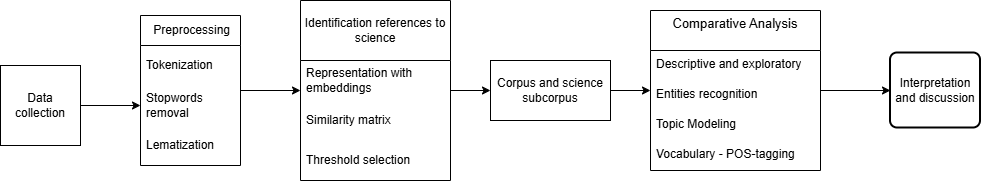
\includegraphics[width=\textwidth]{figures/diagrama_paper_ciencia.png}
		\caption{Distribución de flujo con la metodología aplicada.}
		\label{fig:diagramaflujo}
	\end{figure}
	
	\subsection{Recolección data}
	Se recolectaron 13 mil columnas de opinión de tres medios de comunicación escritos colombianos de alta circulación. Estas fueron publicadas entre enero de 2018 y diciembre de 2020.  En esta fase el único filtro de selección fue que la columna fuera completamente texto y no incluyera video o audio necesario para entender su contenido. Las columnas no se seleccionaron por ningún tema en especifico.
	
	Para cada columna de opinión se recolectaron los siguientes metadatos: el nombre del periódico, el autor, la fecha, el título, el texto (cuerpo) de la columna y el vínculo. Se verificó que cada texto sea único (las columnas no se repiten) y se normalizaron los nombres de los autores. Luego de este proceso se asignaron números de identificación únicos para cada columna de opinión. 
	
	\begin{table}[H]
		\centering
		\caption{Distribución de columnas y autores por periódico}
		\label{tab:col_autores_periodico}
		\footnotesize
		\begin{tabular}{l c c c}
			\hline
			\textbf{Medio} & \textbf{Número de columnas} & \textbf{Número de autores distintos} & \textbf{\% del total de columnas} \\
			\hline
			El Espectador & 10509 & 263 & 76.84\\
			El Tiempo & 1982 &  249 & 14.49\\
			Semana & 1185 & 96  & 8.66\\
			\hline
		\end{tabular}
	\end{table}
	
	\subsection{Preprocesamiento}

		Cuando se trabaja con grandes volúmenes de texto, como en el caso de este corpus de columnas de opinión, el análisis no puede comenzar directamente sobre el material bruto. Es necesario, primero, transformarlo en un formato que pueda ser interpretado por los algoritmos de procesamiento de lenguaje natural (PLN) \cite{Chai2022}. Este proceso de preparación, conocido como preprocesamiento, implica una serie de decisiones metodológicas orientadas a limpiar, estructurar y estandarizar el texto antes de su modelado. En esta investigación, el procedimiento comenzó con una depuración inicial de cada columna, en la que se eliminaron URLs, hashtags y menciones a usuarios de redes sociales (@), así como espacios en blanco redundantes y caracteres distintos de letras, números y signos de puntuación habituales. Esta limpieza permitió reducir ruido y homogeneizar el corpus.

		Una vez depurado el texto, se procedió a segmentarlo en unidades analíticas básicas mediante tokenización. Este paso consiste en dividir el texto en fragmentos más pequeños (denominados tokens) que, en este caso, corresponden a palabras individuales \cite{Tyagi_text}. De este modo, una oración como “La tokenización es elemental” se transforma en la secuencia “La”, “tokenización”, “es” y “elemental”. Esta operación, aparentemente simple, es fundamental porque convierte el texto no estructurado en una estructura manipulable computacionalmente, permitiendo calcular frecuencias, co-ocurrencias y otras métricas lingüísticas.
		

		Posteriormente, y dependiendo de los requerimientos específicos de cada algoritmo aplicado, se eliminaron las denominadas stopwords. Estas son palabras muy frecuentes que cumplen funciones gramaticales (como artículos, preposiciones, pronombres o conjunciones) y que, aunque esenciales para la coherencia sintáctica, suelen aportar poca información semántica en tareas como el modelado de tópicos \cite{Siino2024}. Además de mejorar la calidad interpretativa de los modelos, su eliminación contribuye a reducir la dimensionalidad del corpus, lo cual resulta relevante en términos computacionales. Dado que las listas de stopwords son dependientes del idioma y del contexto analítico, las utilizadas en este estudio fueron revisadas y ajustadas antes de aplicarlas al corpus, particularmente en la etapa previa al modelado de tópicos (véase sección \ref{sec:topic_model}).
		
	
		Finalmente, el proceso incluyó la lematización, es decir, la reducción de las palabras a su forma canónica o lema. Esta estandarización permite agrupar variantes morfológicas bajo una misma entrada léxica, por ejemplo, llevar verbos conjugados a infinitivo o transformar plurales en singular, lo cual resulta crucial en análisis de frecuencia y estudios léxicos \cite{Orellana2018}. La selección del modelo de lematización requirió especial atención. En una primera etapa se utilizó el lematizador de la librería spaCy en Python, cuya principal ventaja es su rapidez; sin embargo, se observaron limitaciones en la precisión para el español. Por esta razón, se optó finalmente por el modelo de la biblioteca Stanford Stanza \cite{qi2020stanza}, basado en redes neuronales, que ofreció mayor exactitud en la identificación de los lemas. La lematización se aplicó antes del análisis léxico y del etiquetado gramatical (POS-tagging), asegurando así una representación más consistente del vocabulario del corpus.

	
	\subsection{Identificación de menciones a la ciencia}
	
	
Para avanzar en el objetivo de esta investigación (comprender cómo se representa la ciencia en el discurso de opinión en Colombia), fue necesario identificar de manera sistemática las menciones asociadas al campo científico dentro del corpus previamente descrito. Para ello, se diseñó una estrategia basada en búsqueda semántica, un método de recuperación de información que permite identificar relaciones de significado más allá de la coincidencia literal de palabras clave \cite{Wei2022}. A diferencia de una búsqueda léxica tradicional, este enfoque recupera textos en función de su proximidad conceptual, incorporando fenómenos como la sinonimia, la variación terminológica y la afinidad semántica entre expresiones.

La estrategia consistió en representar tanto el corpus de aproximadamente 13.000 columnas como las 17 categorías del TESAURO UNESCO para Ciencias mediante embeddings (representaciones vectoriales que capturan el significado contextual de los textos). Cada una de las categorías del Tesauro (concebidas como campos semánticos que agrupan términos representativos de distintas áreas científicas) fue codificada como una consulta semántica (query), compuesta por el conjunto de palabras y expresiones asociadas a dicha categoría. De forma paralela, los fragmentos del corpus fueron transformados en representaciones vectoriales comparables.
	
Una vez obtenidos estos vectores, se calculó la similitud semántica entre cada fragmento del corpus y cada una de las 17 categorías mediante la similitud de coseno (métrica que cuantifica el grado de cercanía entre dos vectores en el espacio semántico). Este procedimiento permitió estimar, para cada fragmento de texto, un conjunto de puntuaciones de afinidad con las distintas categorías del Tesauro. A partir de estas puntuaciones se generó un ranking de similitud y se asignó cada fragmento a la categoría con mayor valor registrado.
	
Como resultado, fue posible identificar no solo qué categorías del campo científico presentan mayor presencia relativa en el corpus de opinión, sino también recuperar fragmentos específicos de columnas clasificados según la categoría con la que muestran mayor proximidad semántica. Estos fragmentos constituyen la base del análisis cualitativo posterior, en el cual se examinan los patrones discursivos asociados a las áreas científicas que registran mayor intensidad semántica en la esfera pública colombiana.

	
	\subsubsection{Definición ciencia: tesauro de la UNESCO}
	Las palabras que se usaron para representar la ciencia son las incluidas en el tesauro de la UNESCO.
	El tesauro de la UNESCO ``es una lista controlada y estructurada de términos para el análisis temático y la búsqueda de documentos y publicaciones en los campos de la educación, cultura, ciencias naturales, ciencias sociales y humanas, comunicación e información.'' \cite{unesco_thesaurus_1977}. 
	Su primera versión en inglés fue publicada en 1977 pero es revisado y actualizado periódicamente. Para este trabajo se usó en particular la lista llamada Ciencia, especializada en ciencias naturales. Esta lista nos permitió acercarnos a la ciencia a partir de las palabras que la componen o se usan para identificarla en diferentes áreas. Esta categoría está compuesta por 17 subcategorías y cada una de ellas contiene entre 24 y 84 términos.
	Para referencia, se incluye una tabla con los primeros términos de cada categoría en la Tabla \ref{tab:categorias_ciencia}.
	
	
	{\footnotesize
		\begin{longtable}{p{3.5cm}P{2cm}p{9cm}}
			\caption{Categorías de Ciencia del Tesauro de la UNESCO y los primeros términos de cada una.} \label{tab:categorias_ciencia}\\
			
			\toprule
			\textbf{Subcategoría} & \textbf{Nº de términos} & \textbf{Primeros 10 términos} \\
			\midrule
			\endfirsthead
			
			\multicolumn{3}{c}{{\bfseries \tablename\ \thetable{} -- continuación}} \\
			\toprule
			\textbf{Subcategoría} & \textbf{Nº de términos} & \textbf{Primeros 10 términos} \\
			\midrule
			\endhead
			
			\midrule \multicolumn{3}{r}{{Continúa en la siguiente página}} \\
			\endfoot
			
			\bottomrule
			\endlastfoot
			
			Enfoque científico & 50 & Análisis causal, Análisis comparativo, Análisis cualitativo, Análisis cuantitativo, Análisis de inspección, Análisis transnacional, Autoevaluación, Calibración, Causa y efecto, Ciencia de la ciencia \\
			
			Administración de la ciencia y de la investigación & 62 & Academia de ciencias, Actividad científica, Administración de la ciencia, Ambientalista, Automatización, Brecha digital, Cambio tecnológico, Centro de investigación, Ciencia y desarrollo, Científico \\
			
			Matemáticas y estadística & 34 & Álgebra, Algoritmo, Análisis de regresión, Análisis de variancia, Análisis estadístico, Análisis factorial, Análisis funcional, Análisis matemático, Análisis multivariado, Análisis numérico \\
			
			Ciencias físicas & 56 & Acústica, Aerodinámica, Calefacción, Calor, Congelación, Conversión de energía, Corriente de agua, Cristalografía, Difusión, Dinámica de fluidos \\
			
			Ciencias químicas & 50 & Acido, Análisis bioquímico, Análisis cromatográfico, Análisis de oligoelementos, Análisis espectroquímico, Análisis químico, Azufre, Carbono, Cinética química, Combustión \\
			
			Ciencias del espacio & 24 & Actividad solar, Agujero negro, Astrofísica, Astronomía, Ciencias del espacio, Cosmología, Espacio, Espacio intersideral, Estrellas, Galaxia \\
			
			Ciencias de la tierra & 61 & Arena, Biogeoquímica, Calor terrestre, Ciencias de la tierra, Conservación del suelo, Corteza terrestre, Cuaternario, Datos geológicos, Depósito de sal, Deriva de los continentes \\
			
			Geografía y oceanografía & 84 & Agua de mar, Aguas costeras, Alta mar, Arrecife de coral, Batimetría, Biogeografía, Biología marina, Carta batimétrica, Ciencia del desierto, Circulación oceánica \\
			
			Meteorología & 34 & Agroclimatología, Atmósfera, Bioclimatología, Ciclo hidrológico, Ciclón, Circulación atmosférica, Clima, Climatología, Condiciones metereológicas, Control meteorológico \\
			
			Hidrología & 46 & Abastecimiento de agua, Agua, Agua del suelo, Agua dulce, Agua potable, Agua salada, Agua salobre, Agua subterránea, Agua superficial, Almacenamiento de agua \\
			
			Ciencias ambientales e ingeniería & 52 & Abastecimiento de energía, Alcantarillado, Aprovechamiento de recursos, Balance energético, Calidad ambiental, Ciencias ambientales, Conservación ambiental, Conservación de la fauna y flora silvestres, Conservación de la energía, Conservación de la naturaleza \\
			
			Polución, catástrofes y seguridad & 54 & Accidente, Adaptación al cambio climático, Agua residual, Alud, Asistencia por desastre, Calentamiento de la tierra, Cambio climático, Contaminación, Contaminación atmosférica, Contaminación del agua \\
			
			Recursos naturales & 53 & Adaptación biológica, Biogás, Bioma, Biomasa, Biosfera, Comportamiento animal, Consumo alimenticio, Crisis ecológica, Diversidad biológica, Ecología animal \\
			
			Biología & 75 & Anatomía, Aparato respiratorio, Bacteria, Bacteriología, Bioética, Biofísica, Biogénesis, Biología, Biología celular, Biología espacial \\
			
			Ciencias naturales & 50 & Alga marina, Animal, Animal acuático, Animal de laboratorio, Animal doméstico, Animal marino, Animal salvaje, Antropología, Árbol, Ave \\
			
			Ciencias médicas & 54 & Acupuntura, Aparato sensorial, Ciencias médicas, Cirugía, Control de alimentos, Dietética, Economía de la salud, Endocrinología, Epidemiología, Estadísticas sanitarias \\
			
			Patología & 40 & Cáncer, Ceguera, Daltonismo, Deficiencia mental, Enfermedad, Enfermedad cardiovascular, Enfermedad de la piel, Enfermedad del sistema nervioso, Enfermedad mental, Enfermedad nutricional \\
			
		\end{longtable}
	}
	
	
	\subsubsection{Selección modelo de embeddings}
Para este trabajo se optó por utilizar un modelo de embeddings preentrenado. Esto significa que el modelo fue desarrollado y entrenado previamente con grandes volúmenes de datos textuales, lo que le permite capturar relaciones semánticas complejas sin necesidad de ser entrenado nuevamente desde cero. Esta estrategia se inscribe en el marco del transfer learning, en el cual un modelo entrenado en una tarea general puede reutilizarse eficazmente en contextos distintos \cite{Hosna2022}. De este modo, fue posible analizar el corpus de columnas de opinión aprovechando conocimiento lingüístico previamente aprendido, reduciendo costos computacionales y tiempos de desarrollo.

La selección del modelo de embeddings requirió considerar varios criterios fundamentales. En primer lugar, era indispensable que el modelo estuviera optimizado para tareas de similitud semántica, dado que el objetivo central era medir la cercanía conceptual entre fragmentos del corpus y las categorías del TESAURO UNESCO para Ciencias. En segundo lugar, debía incluir adecuadamente el idioma español, puesto que el corpus analizado corresponde a columnas de opinión en Colombia. Finalmente, se evaluó el tamaño del modelo (entendido como el número de parámetros y el requerimiento de memoria), procurando que no superara los 500 millones de parámetros para garantizar viabilidad computacional.

La decisión final se apoyó en los resultados del Massive Multilingual Text Embedding Benchmark (MMTEB), una evaluación comparativa a gran escala de modelos de embeddings multilingües desarrollada por \cite{enevoldsen2025mmtebmassivemultilingualtext}. Este benchmark permite comparar el desempeño de distintos modelos en tareas como recuperación de información y similitud semántica. Entre los modelos evaluados, uno de los que mejor equilibró rendimiento en español, desempeño en tareas de similitud y tamaño moderado fue embeddinggemma-300m, desarrollado por Google \cite{vera2025embeddinggemmapowerfullightweighttext}. Este modelo cuenta con aproximadamente 300 millones de parámetros y admite una ventana de contexto de hasta 2048 tokens, lo que lo hace adecuado para procesar fragmentos de texto relativamente extensos sin perder coherencia semántica.

Una vez seleccionado el modelo, se procedió a preparar el corpus para la codificación vectorial. Dado que las columnas de opinión suelen abordar múltiples temas en un mismo texto, trabajar con documentos completos dificultaría la identificación precisa de menciones a la ciencia. Por esta razón, cada columna fue dividida en fragmentos (chunks) de aproximadamente 150 palabras, estableciendo un mínimo de 100 palabras y un solapamiento de 20 palabras entre fragmentos consecutivos. La definición de un tamaño mínimo es relevante porque la fragmentación se realiza secuencialmente desde el inicio del texto, lo que puede generar un último fragmento excesivamente corto; cuando esto ocurría, dicho fragmento se integraba al anterior. El solapamiento entre fragmentos (es decir, que cada nuevo segmento comience algunas palabras antes de que finalice el anterior) permite preservar continuidad contextual y evitar cortes abruptos en el significado. Además, este procedimiento garantiza que cada fragmento permanezca dentro del límite máximo de tokens admitido por el modelo.

Posteriormente, se calculó el embedding representativo de cada fragmento del corpus. De manera análoga, para cada subcategoría del TESAURO UNESCO se construyó un texto compuesto por la concatenación de sus palabras clave, y sobre esa cadena se generó el embedding correspondiente. Así, tanto los fragmentos de las columnas como las categorías del Tesauro quedaron representados en un mismo espacio vectorial.

Finalmente, se estimó la similitud semántica entre cada fragmento del corpus y cada subcategoría del Tesauro mediante el cálculo de la similitud de coseno, con el fin de identificar el grado de cercanía conceptual entre ambos. En la siguiente sección se explicará con mayor detalle el fundamento matemático de la similitud de coseno y su interpretación en el contexto de este análisis.

	
	\subsubsection{Similitud de coseno}
	
	Una vez representados tanto los fragmentos del corpus como las subcategorías del TESAURO UNESCO en el mismo espacio vectorial mediante embeddings, fue necesario definir una métrica que permitiera cuantificar su cercanía semántica. La medida utilizada para evaluar la similaridad entre los textos codificados fue la similitud de coseno, una de las métricas más empleadas en recuperación de información y procesamiento de lenguaje natural (\cite{Jurafsky2025}).
		
	En este contexto, sea $\mathbf{u}$ el vector correspondiente a un fragmento (chunk) de una columna de opinión, y sea $\mathbf{v}$ el vector asociado a una de las 17 categorías del Tesauro UNESCO para Ciencias. La similitud de coseno entre ambos vectores se define como:
		
	\begin{equation}
			\text{sim}_{\cos}(\mathbf{u}, \mathbf{v}) =
			\frac{\mathbf{u} \cdot \mathbf{v}}
			{|\mathbf{u}| , |\mathbf{v}|}
	\end{equation}
		
	donde $\mathbf{u} \cdot \mathbf{v}$ representa el producto punto entre los vectores, y $|\mathbf{u}|$ y $|\mathbf{v}|$ corresponden a sus normas euclidianas. Esta expresión calcula el coseno del ángulo formado entre ambos vectores en el espacio semántico.
		
	El valor de esta medida oscila entre -1 y 1. Un valor cercano a 1 indica que los vectores apuntan en la misma dirección (ángulo cercano a 0 grados), lo que implica alta similitud semántica. Un valor cercano a 0 indica ortogonalidad (ángulo cercano a 90 grados), es decir, ausencia de relación semántica significativa. Un valor cercano a -1 correspondería a vectores en direcciones opuestas (ángulo cercano a 180 grados), lo que en términos semánticos implicaría oposición o disimilitud extrema. En la práctica, cuando se trabaja con embeddings generados por modelos de lenguaje modernos, los valores suelen concentrarse en el rango $[0,1]$ debido a la naturaleza de las representaciones.
		
	En el procedimiento implementado en esta investigación, para cada fragmento $\mathbf{u}$ del corpus se calculó su similitud de coseno con cada uno de los 17 vectores $\mathbf{v}$ correspondientes a las categorías del Tesauro. Esto permitió obtener, para cada fragmento, un conjunto de 17 puntuaciones de afinidad semántica. La categoría asignada al fragmento fue aquella que registró el mayor valor de similitud. De esta manera, cada chunk de las columnas de opinión quedó clasificado según el campo científico con el cual presenta mayor proximidad conceptual.
	

	\subsubsection{Umbral de selección}

Una vez segmentado el corpus completo de columnas de opinión, se obtuvieron en total $m = 62\,651$ fragmentos (chunks). Cada uno de estos fragmentos fue representado mediante un \emph{embedding} y comparado con los $n = 17$ vectores correspondientes a las categorías del TESAURO UNESCO para Ciencias. En consecuencia, el índice $i$ recorre los fragmentos del corpus ($i = 1, \dots, 62\,651$) y el índice $j$ recorre las categorías del Tesauro ($j = 1, \dots, 17$).

Para cada par $(i,j)$ se calculó la similitud de coseno entre el \emph{embedding} del fragmento texto $i$ y el \emph{embedding} de la categoría $j$. Este procedimiento produjo una matriz de similitud $\mathbf{S} \in \mathbb{R}^{m \times n}$, definida como:

\begin{equation}
	\mathbf{S} =
	\begin{bmatrix}
		s_{1,1} & s_{1,2} & s_{1,3} & \cdots & s_{1,n} \\
		s_{2,1} & s_{2,2} & s_{2,3} & \cdots & s_{2,n} \\
		s_{3,1} & s_{3,2} & s_{3,3} & \cdots & s_{3,n} \\
		\vdots  & \vdots  & \vdots  & \ddots & \vdots  \\
		s_{m,1} & s_{m,2} & s_{m,3} & \cdots & s_{m,n}
	\end{bmatrix}
\end{equation}

donde cada elemento

\[
s_{i,j} = \text{sim}_{\cos}(\text{texto i}, \text{categoría j})
\]

representa el grado de proximidad semántica entre el fragmento $i$ y la categoría $j$.

A partir de esta matriz, para cada fragmento $i$ se identificó la categoría con mayor valor de similitud, es decir,

\[
j^*(i) = \arg\max_{j \in \{1,\dots,17\}} s_{i,j}.
\]

Sin embargo, este criterio de asignación implica que todo fragmento queda clasificado en alguna categoría, incluso cuando sus niveles de similitud son bajos en términos absolutos. En otras palabras, el procedimiento de máximo relativo no distingue entre fragmentos que presentan una afinidad semántica significativa con el campo científico y aquellos cuya cercanía es débil o incidental.

Por esta razón, se introdujo un umbral de selección. Sea $\tau \in [0,1]$ dicho umbral. Un fragmento $i$ se considera una mención efectiva de ciencia únicamente si

\[
\max_{j} s_{i,j} \geq \tau.
\]

En caso contrario, el fragmento no se clasifica como mención científica, aun cuando tenga asignada una categoría por el criterio de máximo relativo. La definición adecuada de este umbral resulta crucial, pues permite maximizar la diferencia entre fragmentos que contienen referencias sustantivas al campo científico y aquellos que no lo hacen.

Para determinar el valor adecuado del umbral $\tau$, se realizó una validación manual basada en lectura cercana de una muestra de fragmentos. El propósito de esta lectura fue construir una clasificación de referencia que permitiera evaluar si los fragmentos identificados automáticamente por medio de la similitud de cosenos como menciones científicas efectivamente lo eran desde un punto de vista interpretativo.

Como paso previo, se examinó la distribución empírica de los puntajes de similitud máxima $j^*(i)$ y se observó que valores inferiores a 0.4 tendían a corresponder a asociaciones semánticas débiles. Con base en esta inspección exploratoria, se fijó 0.4 como punto de corte inicial para construir la muestra de validación.

Se filtraron entonces los fragmentos cuyo puntaje máximo de similitud fuera superior a 0.4. A partir de este subconjunto se seleccionaron aleatoriamente 10 fragmentos por cada una de las 17 categorías del Tesauro, obteniendo un total de 170 fragmentos. Cada uno fue leído y clasificado manualmente como “mención efectiva de ciencia” o “no mención”, según si el contenido del fragmento correspondía de manera sustantiva al campo científico asignado.

Esta clasificación manual permitió comparar la asignación automática con la evaluación humana. En el procedimiento automático, cada fragmento se asocia a la categoría con mayor similitud $j^*(i)$, pero solo se considera una mención efectiva de ciencia si el valor máximo de similitud $\max_j s_{i,j}$ supera el umbral $\tau$. El accuracy se calculó como la proporción de coincidencias entre la clasificación manual de referencia y la decisión automática (asignación y validación por umbral). Al evaluar distintos valores de $\tau$, fue posible identificar el punto que maximiza la concordancia entre el procedimiento computacional y la lectura interpretativa.

La figura~\ref{fig:resultados-clasificacion} muestra la evolución del \emph{accuracy} en función del umbral $\tau$ utilizado para decidir si un fragmento del corpus constituye una mención efectiva de ciencia. En el eje horizontal se representan los distintos valores posibles del umbral, mientras que en el eje vertical se presenta el nivel de concordancia entre la clasificación automática y la clasificación manual de referencia. Cada punto de la curva corresponde al \emph{accuracy} obtenido al aplicar un valor específico de $\tau$ sobre la muestra de validación. La gráfica permite observar cómo cambia el desempeño del modelo a medida que el criterio de decisión se vuelve más o menos exigente.

Por ejemplo, si se fija el umbral en $\tau = 0.47$, un fragmento se clasifica como mención científica únicamente cuando su similitud máxima con alguna de las 17 categorías del Tesauro satisface

\[
\max_j s_{i,j} \ge 0.47.
\]

Al aplicar este criterio sobre los 170 fragmentos evaluados manualmente, se obtiene un \emph{accuracy} cercano a 0.74. Esto significa que aproximadamente el 74\% de las decisiones automáticas coinciden con la clasificación realizada mediante lectura cercana. En términos prácticos, el modelo reproduce el juicio humano en casi tres de cada cuatro casos. Este valor representa un punto de equilibrio: si el umbral fuera menor, se incluirían asociaciones semánticas débiles; si fuera mayor, se excluirían fragmentos que sí contienen menciones sustantivas a la ciencia.
	
Con el umbral seleccionado, el procedimiento se aplicó al conjunto completo de $62\,651$ fragmentos del corpus, lo que permitió identificar un subcorpus compuesto por $7\,267$ \emph{chunks} que cumplen el criterio de mención efectiva de ciencia. Este subcorpus constituye la base para los análisis temáticos posteriores.


	
\begin{figure}[H]
	\centering
	\begin{subfigure}{0.48\textwidth}
		\centering
		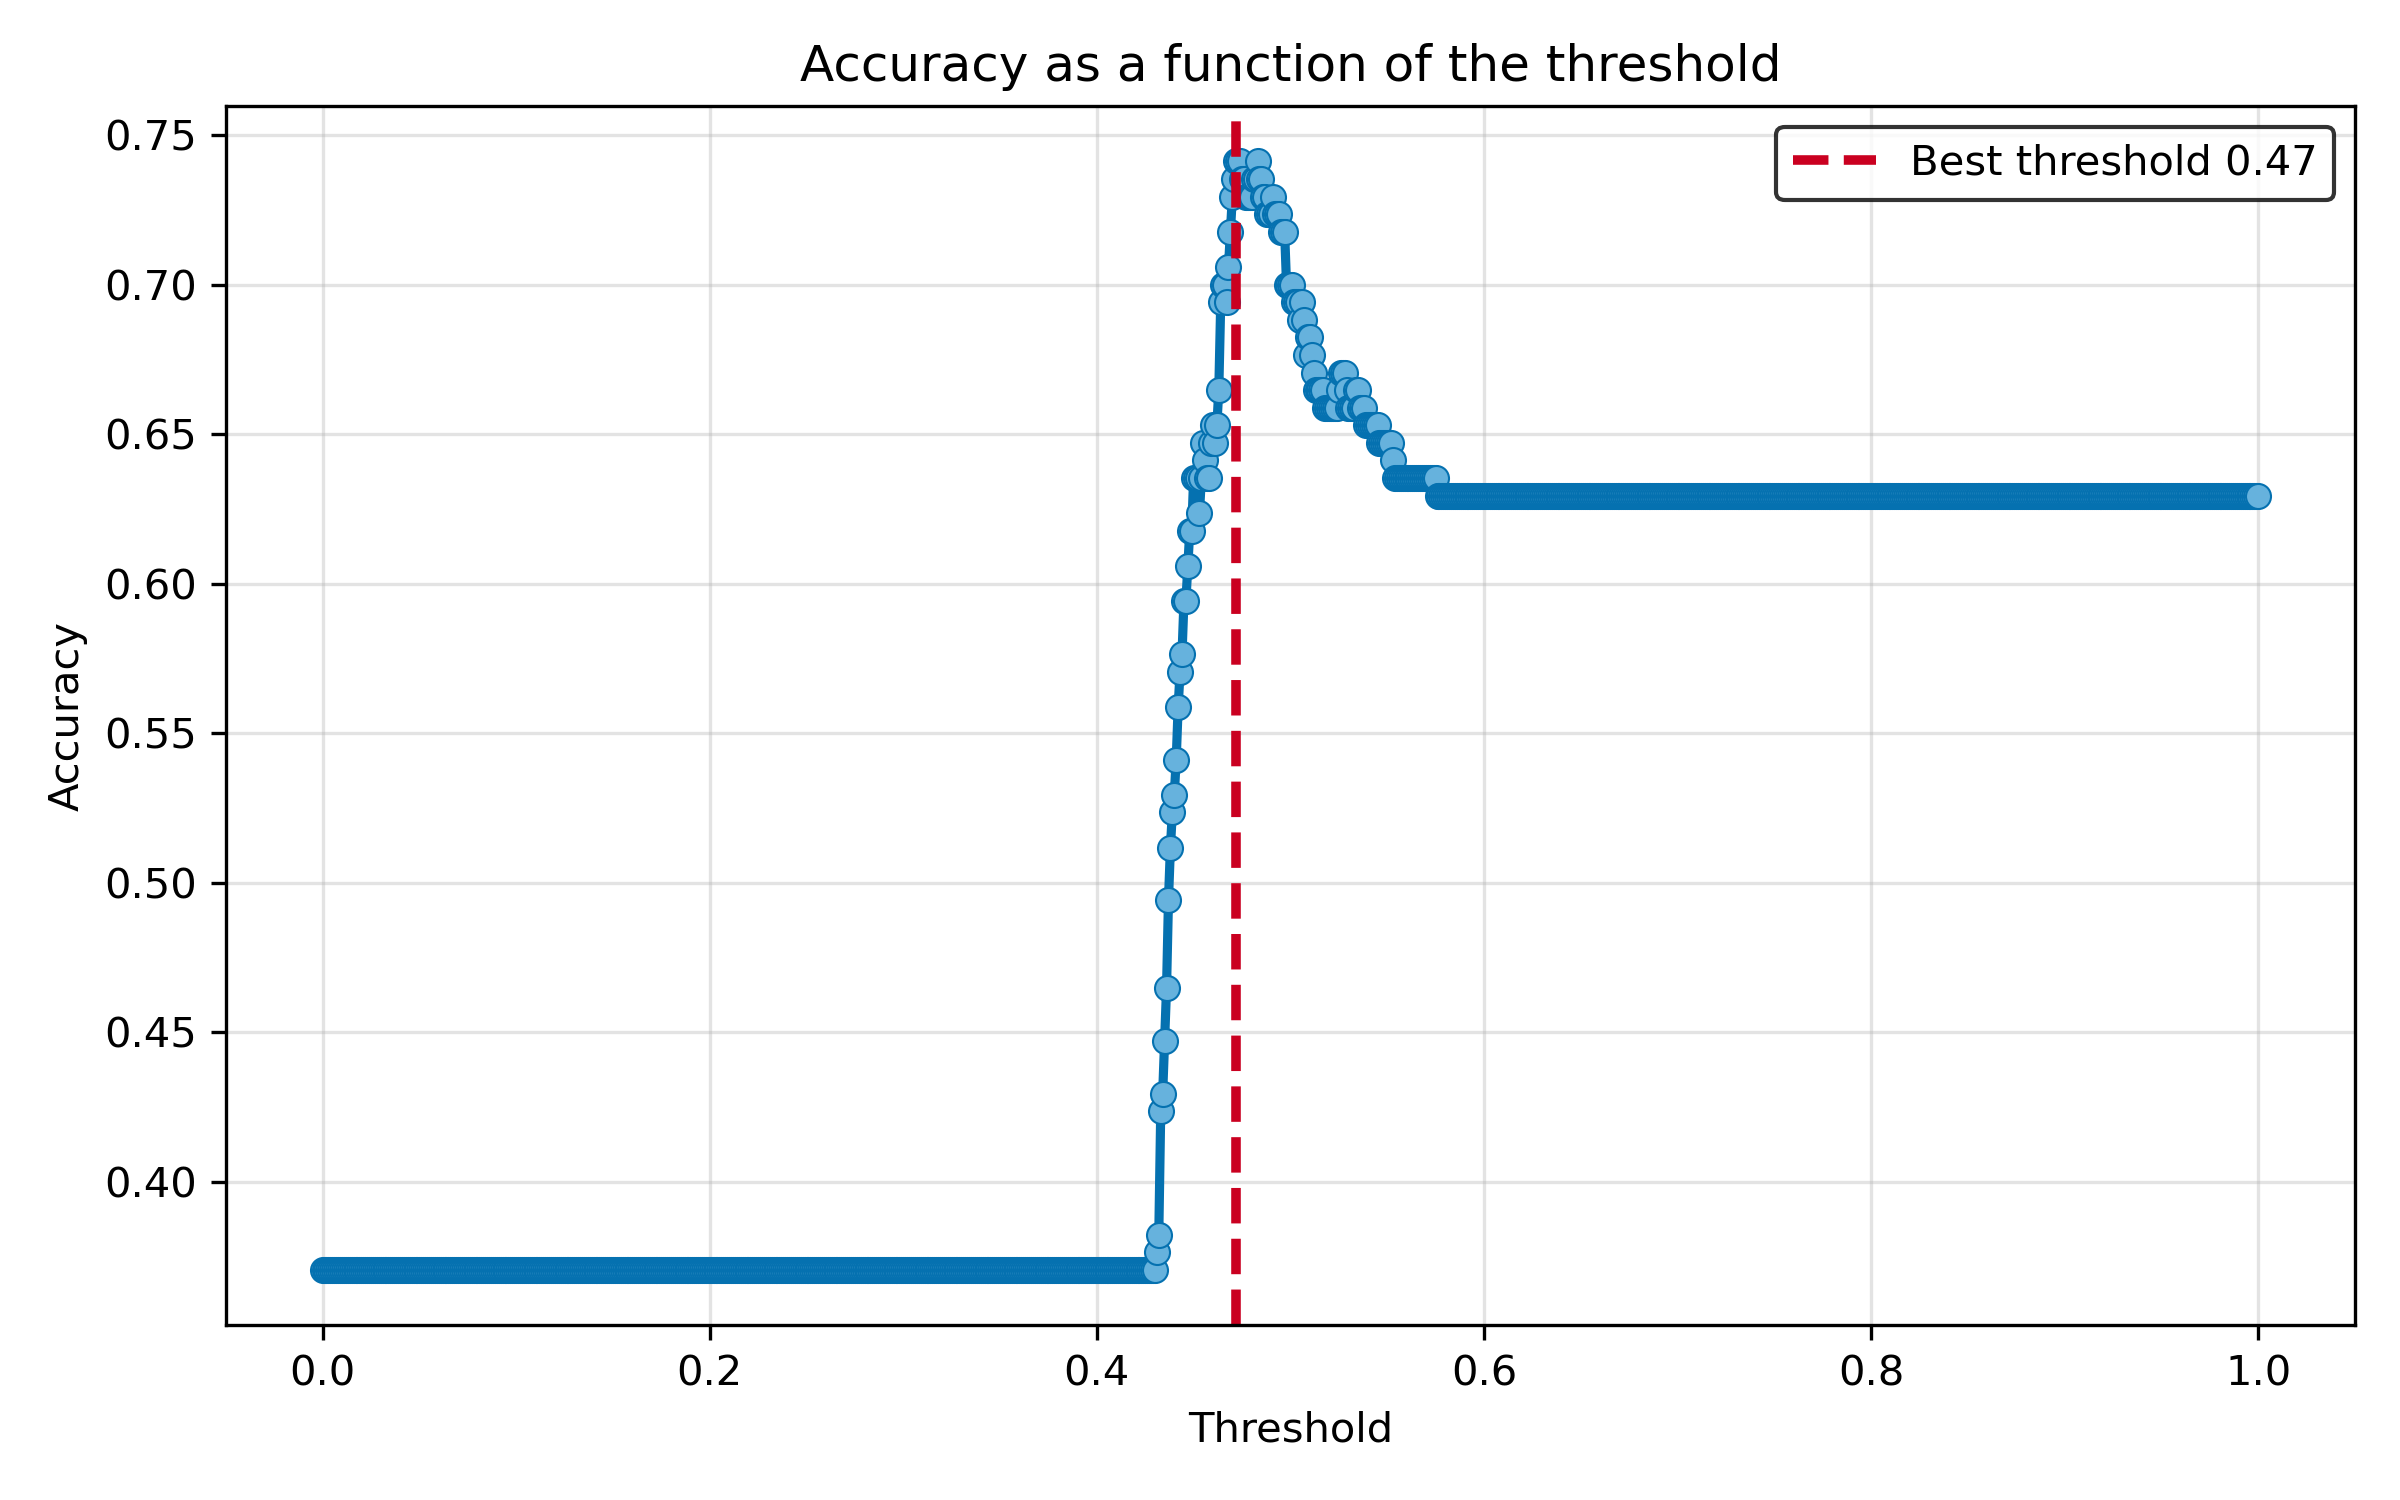
\includegraphics[width=\textwidth]{figures/accuracy_umbral.png}
		\caption{Accuracy por umbral.}
		\label{fig:accuracy-umbral}
	\end{subfigure}
	\caption{Resultados de análisis de clasificación: distribución de scores y precisión según umbral.}
	\label{fig:resultados-clasificacion}
\end{figure}


\subsection{Análisis descriptivos y exploratorios del texto}
	
	
	Para caracterizar el corpus y establecer una base adecuada para los análisis posteriores, se llevó a cabo un procedimiento de descripción general mediante el cálculo de diversos estadísticos. Entre ellos se incluyeron el número total de palabras, la cantidad de palabras únicas, así como la longitud máxima y mínima por columna (documento). Estos indicadores permiten dimensionar la estructura y amplitud del conjunto de textos antes de avanzar hacia análisis más específicos.
	
	Asimismo, con el propósito de obtener una aproximación exploratoria al contenido discursivo, se generaron dos nubes de palabras: una correspondiente al corpus completo y otra al subcorpus de ciencia. Para su construcción se aplicó un preprocesamiento que involucró limpieza textual, normalización y tokenización. Las nubes se elaboraron a partir de las frecuencias de términos, facilitando una comparación preliminar de los vocabularios predominantes en cada conjunto.
	
	Finalmente, se desarrolló un análisis temporal basado en el cálculo del volumen mensual de documentos y en la identificación de aquellos que contienen menciones asociadas a ciencia. Este procedimiento permitió estructurar una serie cronológica destinada a examinar las dinámicas temporales de la presencia temática en etapas posteriores del análisis.
	
	
	
	\subsection{Análisis de entidades – NER}
	El reconocimiento de entidades nombradas (NER, por sus siglas en inglés) es una tarea del procesamiento del lenguaje natural que consiste en identificar las entidades mencionadas en un texto y clasificarlas en categorías preestablecidas (por ejemplo, personas, lugares u organizaciones) \cite{Jehangir2023}. Este proceso desempeña un papel fundamental en diversos ámbitos, como el análisis de redes sociales, la anotación semántica, la traducción automática, los sistemas de preguntas y respuestas, el resumen automático de texto, la clasificación documental, la detección de spam y la minería de opiniones \cite{Jehangir2023}.
	
	En este trabajo se aplicó un modelo de reconocimiento de entidades nombradas a todo el corpus, y posteriormente se realizó un análisis comparativo con el subcorpus de ciencia. Para ello, se calculó la frecuencia de aparición de cada entidad en ambos corpus y se obtuvo el cociente que indica en qué medida una entidad aparece con mayor frecuencia en textos relacionados con ciencia que en el resto del corpus.
	
	El modelo utilizado fue Babelscape/wikineural-multilingual-ner \cite{tedeschi-etal-2021-wikineural-combined}, disponible en la librería Sentence Transformers. Este modelo presenta métricas sólidas y está preentrenado con datos que incluyen el español. Reconoce lugares, personas y organizaciones, y agrupa en una categoría miscelánea aquellas entidades que no se ajustan a estos tipos.
	
	\subsection{Análisis de temas}\label{sec:topic_model}
	
	
	Una vez identificadas las menciones a la ciencia y construido el subcorpus correspondiente, se procedió al modelado de tópicos con el fin de inferir las estructuras temáticas latentes presentes tanto en el corpus general como en el subcorpus científico. El modelado de tópicos es un conjunto de métodos no supervisados cuyo objetivo es descubrir patrones semánticos recurrentes en una colección de documentos \cite{Abdelrazek2023}. En términos conceptuales, estos métodos buscan modelar tres entidades fundamentales: la colección de documentos, los tópicos latentes y los constructos que los conforman. En este contexto, los constructos corresponden a las unidades léxicas (palabras o términos) que componen los fragmentos analizados.
	
	Desde un punto de vista matemático, un tópico puede entenderse como una distribución de probabilidad sobre el vocabulario del corpus. Es decir, dado un conjunto de palabras $w_1, w_2, \dots, w_V$ que conforman el vocabulario, un tópico $k$ se representa como un vector de probabilidades
	
	\[
	\boldsymbol{\phi}_k = \left( P(w_1 \mid k), P(w_2 \mid k), \dots, P(w_V \mid k) \right),
	\]
	
	donde $P(w_v \mid k) \ge 0$ y
	
	\[
	\sum_{v=1}^{V} P(w_v \mid k) = 1.
	\]
	
	Por ejemplo, un tópico asociado al campo de la salud podría asignar mayor probabilidad a términos como \emph{vacuna}, \emph{epidemia}, \emph{hospital} o \emph{salud pública}, mientras que otras palabras del vocabulario recibirían probabilidades cercanas a cero. De esta forma, el tópico no se define por una única palabra, sino por una estructura probabilística que describe la relevancia relativa de los términos dentro de ese tema latente.
	
	En la literatura se han desarrollado cuatro grandes familias de métodos para el modelado de tópicos: algebraicos, difusos, probabilísticos y neuronales. Los modelos algebraicos, surgidos en la década de 1990, constituyeron los primeros intentos sistemáticos por identificar estructuras temáticas a partir de descomposiciones matriciales. Más recientemente, los enfoques neuronales han concentrado mayor atención debido a su capacidad para capturar relaciones semánticas complejas. Entre ellos destaca BERTopic \cite{Grootendorst2022}, que combina embeddings preentrenados, reducción de dimensionalidad y algoritmos de clustering para identificar grupos de documentos con alta proximidad semántica.
	
	Dado que en las etapas anteriores del análisis ya se emplearon embeddings para representar los fragmentos del corpus, se optó por mantener coherencia metodológica utilizando el mismo modelo de representación vectorial (embeddinggemma-300m) en el modelado de tópicos. Esto garantiza que la estructura semántica capturada en la identificación de menciones científicas se preserve también en la inferencia temática.
	
	El modelo se aplicó tanto al corpus completo como al subcorpus de ciencia, lo que permitió realizar posteriormente comparaciones entre las configuraciones temáticas generales y aquellas específicamente asociadas al discurso científico. La implementación en Python permitió controlar diversos componentes del proceso, incluyendo el modelo de embeddings, el número máximo de tópicos a estimar y el número mínimo de documentos requeridos para conformar un tópico. Asimismo, se aplicó una reducción de \emph{outliers} con el fin de disminuir la cantidad de fragmentos no asignados y forzar una clasificación más exhaustiva.
	
	Para evaluar la calidad de los tópicos estimados, se utilizó la métrica de coherencia temática. Esta medida, basada en principios probabilísticos de coocurrencia entre términos, ha mostrado correlación positiva con la interpretabilidad humana de los tópicos \cite{Rder2015}. Con el propósito de seleccionar el número óptimo de tópicos, el modelo se ejecutó con distintos valores de este parámetro y se calculó la coherencia correspondiente en cada caso. El valor que maximizó dicha métrica se adoptó como configuración final del modelo.


	\subsection{Análisis de vocabulario con POS-tagging}
	Con el fin de identificar el vocabulario más relevante asociado al discurso sobre ciencia en las columnas de opinión, se realizó un análisis de frecuencia de verbos, adjetivos y sustantivos tanto en el corpus general como en el subcorpus de ciencia. Para obtener estas categorías gramaticales se empleó un modelo de Part-of-Speech Tagging (POS-tagging). Esta tarea consiste en asignar a cada palabra su categoría sintáctica correspondiente (sustantivo, verbo, adjetivo, preposición, entre otras) \cite{he2020surveyrecentadvancessequence}. El POS-tagging constituye un componente fundamental en diversas aplicaciones del procesamiento del lenguaje natural, tales como traducción automática, recuperación y extracción de información, análisis sintáctico, desambiguación semántica y análisis de sentimientos \cite{Chiche2022}.
	
	Para este trabajo se utilizó el POS-tagger de Stanza, un paquete de análisis lingüístico para Python que incluye modelos entrenados para múltiples idiomas, entre ellos el español \cite{qi2020stanzapythonnaturallanguage}. Este modelo fue seleccionado debido a sus métricas de desempeño reportadas y a su adecuación para textos periodísticos. En el corpus analizado mostró un comportamiento consistente, permitiendo extraer de manera fiable las clases gramaticales necesarias para el análisis comparativo de frecuencias.
	
	\section{Resultados}


En esta sección se presentan los resultados derivados del procedimiento metodológico descrito anteriormente, siguiendo la misma secuencia analítica. En primer lugar, se reporta la identificación de menciones efectivas a la ciencia y la delimitación del subcorpus correspondiente. Posteriormente, se exponen análisis descriptivos y exploratorios que caracterizan cuantitativamente su presencia en el corpus. A continuación, se presentan los resultados del reconocimiento de entidades nombradas, con el fin de identificar actores e instituciones asociados al discurso científico. Seguidamente, se muestran los hallazgos del modelado de tópicos, que permiten inferir las estructuras temáticas latentes tanto en el corpus general como en el subcorpus de ciencia. Finalmente, se analizan patrones léxicos y gramaticales mediante técnicas de \emph{POS-tagging}, lo que contribuye a una comprensión más detallada de la forma lingüística que adopta la representación de la ciencia en la esfera pública.

	
	\subsection{Identificación de menciones a la ciencia}\label{sec:ident_menciones}


A partir de la clasificación manual de 170 fragmentos utilizados para validación, se determinó que un umbral adecuado es $\tau = 0.47$, con el cual se obtuvo un \emph{accuracy} de 0.741. Una vez fijado este criterio, el procedimiento se aplicó al conjunto completo de 13\,676 columnas de opinión, las cuales fueron segmentadas en 62\,651 fragmentos. De estos, 7\,267 fragmentos fueron identificados como relacionados con la ciencia, lo que representa el 11.6\% del total de fragmentos.

En términos de documento completo, 4\,154 columnas contienen al menos una mención efectiva a la ciencia, lo que equivale al 30.4\% del total de columnas analizadas. La Tabla~\ref{tab:res_fragmentos_subcategoria} presenta la distribución de los fragmentos clasificados como menciones científicas en las 17 categorías del TESAURO UNESCO.
	
	
	{\footnotesize
		\begin{longtable}{p{7cm}P{4cm}P{4cm}}
			\caption{Cantidad de fragmentos con menciones a la ciencia con porcentaje respecto al total por categoría} \label{tab:res_fragmentos_subcategoria}\\
			\toprule
			\textbf{Subcategoría} & \textbf{Número de fragmentos} & \textbf{Porcentaje del total} \\
			\midrule
			\endfirsthead
			
			\multicolumn{3}{c}{{\bfseries \tablename\ \thetable{} -- continuación}} \\
			\toprule
			\textbf{Categoría} & \textbf{Número de fragmentos} & \textbf{Porcentaje del total} \\
			\midrule
			\endhead
			
			\midrule \multicolumn{3}{r}{{Continúa en la siguiente página}} \\
			\endfoot
			
			\bottomrule
			\endlastfoot
			
			Administración de la ciencia y de la investigación & 3195 & 43.97\% \\
			Polución, catástrofes y seguridad & 1566 & 21.55\% \\
			Ciencias ambientales e ingeniería & 635 & 8.74\% \\
			Ciencias naturales & 470 & 6.47\% \\
			Patología & 375 & 5.16\% \\
			Ciencias médicas & 306 & 4.21\% \\
			Matemáticas y estadística & 250 & 3.44\% \\
			Hidrología & 104 & 1.43\% \\
			Recursos naturales & 68 & 0.94\% \\
			Enfoque científico & 64 & 0.88\% \\
			Ciencias del espacio & 61 & 0.84\% \\
			Geografía y oceanografía & 49 & 0.67\% \\
			Biología & 36 & 0.50\% \\
			Meteorología & 28 & 0.39\% \\
			Ciencias de la tierra & 23 & 0.32\% \\
			Ciencias físicas & 20 & 0.28\% \\
			Ciencias químicas & 17 & 0.23\% \\
			\midrule
			\textbf{Total} & \textbf{7267} & \textbf{100\%} \\
		\end{longtable}
	}
	
	 
	
	A  continuación se incluyen algunos ejemplos de los fragmentos seleccionados. \textcolor{green}{Poner los originales en material suplementario, acá se ponen los traducidos al inglés, si no has visto en la revisión de la literatura una mejor opción de mostrarlos, además deberíamos compartir el enlace de donde los tomamos y mencionar la línea en donde empieza y donde termina la referencia en el texto original}\\
	 
	
	De la categoría: Administración de la ciencia y de la investigación
	
	\begin{quote}
		(...) separado. El Ministerio de Ciencia, Tecnología e Innovación tiene la responsabilidad de convocar la constitución de un Sistema Nacional de Innovación que asuma como propósito desarrollar la hoja de ruta planteada por la Misión de Sabios, alineando a todos los actores a nivel local, regional y nacional. El conocimiento siempre es un logro colectivo. Frente a los desafíos que afrontamos como país, es necesario que asumamos colectivamente, todos los actores, el reto de gestionar el conocimiento, aprendiendo de manera continua, para ponerlo al servicio de las comunidades. Para superar la crisis y lograr las transformaciones estructurales se requiere planeación y un trabajo de mediano y largo plazo, en donde todos sumemos sin pensar solo en réditos inmediatos. Un sistema en donde el arte, las humanidades, la tecnología y las ciencias sociales y exactas, como expresión del conocimiento, hagan parte de la cotidianidad de los colombianos nos exige dejar de actuar (...)
	\end{quote}
	
	De la categoría Ciencias ambientales e ingeniería
	
	\begin{quote}
		(...) la justicia ambiental y climática. 4. Articular los objetivos de desarrollo sostenible y la agenda 2030 del posconflicto, focalizándonos en energías renovables, transporte multimodal, bioconstrucción, permacultura, autoconsumo y territorios hídricos resilientes. 5. Redefinir la relación urbanorural, enfatizando restauración y conservación de ecosistemas, equidad, solidaridad, corresponsabilidad e identidad. 6. Revisar el modelo mineroenergético ajustándolo al ordenamiento ambiental territorial, no construir nuevos megaproyectos hidroeléctricos, negar el uso del fracking y hacer transición energética hacia energías renovables alternativas. 7. Promover la educación integral y la democratización de la información y el conocimiento como instrumentos de construcción de la paz, respetando las utopías y las diversidades culturales y naturales. 8. Fortalecer la investigación científica, la innovación y otros modos de construcción del conocimiento como medios para mejorar el conocimiento de la realidad ecológica, climática y cultural. 9. Reconocer a la naturaleza como víctima del conflicto armado y del modelo de desarrollo colombiano, y, por (...)
	\end{quote}
	
	De la categoría Matemáticas y estadística
	
	\begin{quote}
		(...) la ciencia aspira a los modelos económicos, a reducirlo todo a un cuerpo teórico pequeño de donde se puedan desprender, por deducción directa, sus corolarios básicos. En matemáticas, digamos, es más bella una demostración corta y aritmética que otra más larga que deba recurrir al cálculo para demostrar lo mismo. Todas las geometrías se desarrollan a partir de un puñado de postulados elementales. Los físicos sueñan con la Teoría del Todo están hartos de lidiar con ese enjambre de partículas empalagosas. ¡Eso no es elegante!. En ciencia, como en arte, lo bello es lo breve, lo simple, así haya siempre una secreta complejidad escondida entre los pliegues. Sí, dedicaré lo mejor de mis días a la búsqueda de la fragancia madre y cuando la encuentre la envasaré en un frasquito que será una gema discreta, claro, y la pondré a los pies de mi esposa, lo prometo. El resto será (...)
	\end{quote}
	
	De la categoría Ciencias químicas
	
	\begin{quote}
		(...) a la formación en ciencias de la naturaleza sabemos que el conocimiento científico y tecnológico tiene unos efectos sociales, económicos y políticos que se deben analizar rigurosamente para que nuestros estudiantes fundamenten su formación ciudadana de manera amplia y crítica, de tal manera que cuenten con las herramientas conceptuales y metodológicas para participar activamente en la vida social. Por ejemplo, cuando estudiamos el tema de hidrocarburos, no solo debemos entender su disposición en la naturaleza, sus propiedades y estructuras químicas, sino también analizar su importancia social, los procesos de explotación y los usos sociales que, en su mayoría, están asociados a la generación de energía a partir de la mezcla de hidrocarburos más famosa que conocemos en el mundo y que denominamos petróleo; al estudiar este tema no solo debemos comprenderlo científicamente, sino considerar simultáneamente que esta mezcla de sustancias orgánicas representa el componente central de la matriz energética del (...)
	\end{quote}
	
	
	
	\subsection{Análisis descriptivos y exploratorios}
	
	\begin{table}[H]
		\centering
		\caption{Estadísticos descriptivos generales del corpus}
		\label{tab:estadisticos_generales}
		\begin{tabular}{l c}
			\hline
			\textbf{Estadístico} & \textbf{Valor} \\
			\hline
			Número total de documentos & 13676\\
			Palabras totales & 8607473\\
			Promedio palabras por documento & 629\\
			Mediana palabras por documento & 590\\
			Máximo palabras por documento & 5223\\
			Mínimo palabras por documento & 128\\
			Número de autores distintos & 584\\
			Número de medios de comunicación distintos & 3\\
			Número de palabras únicas (vocabulario total) & 283923\\
			\hline
		\end{tabular}
	\end{table}
	
		\begin{figure}[H]
		\centering
		\begin{subfigure}{0.48\textwidth}
			\centering
			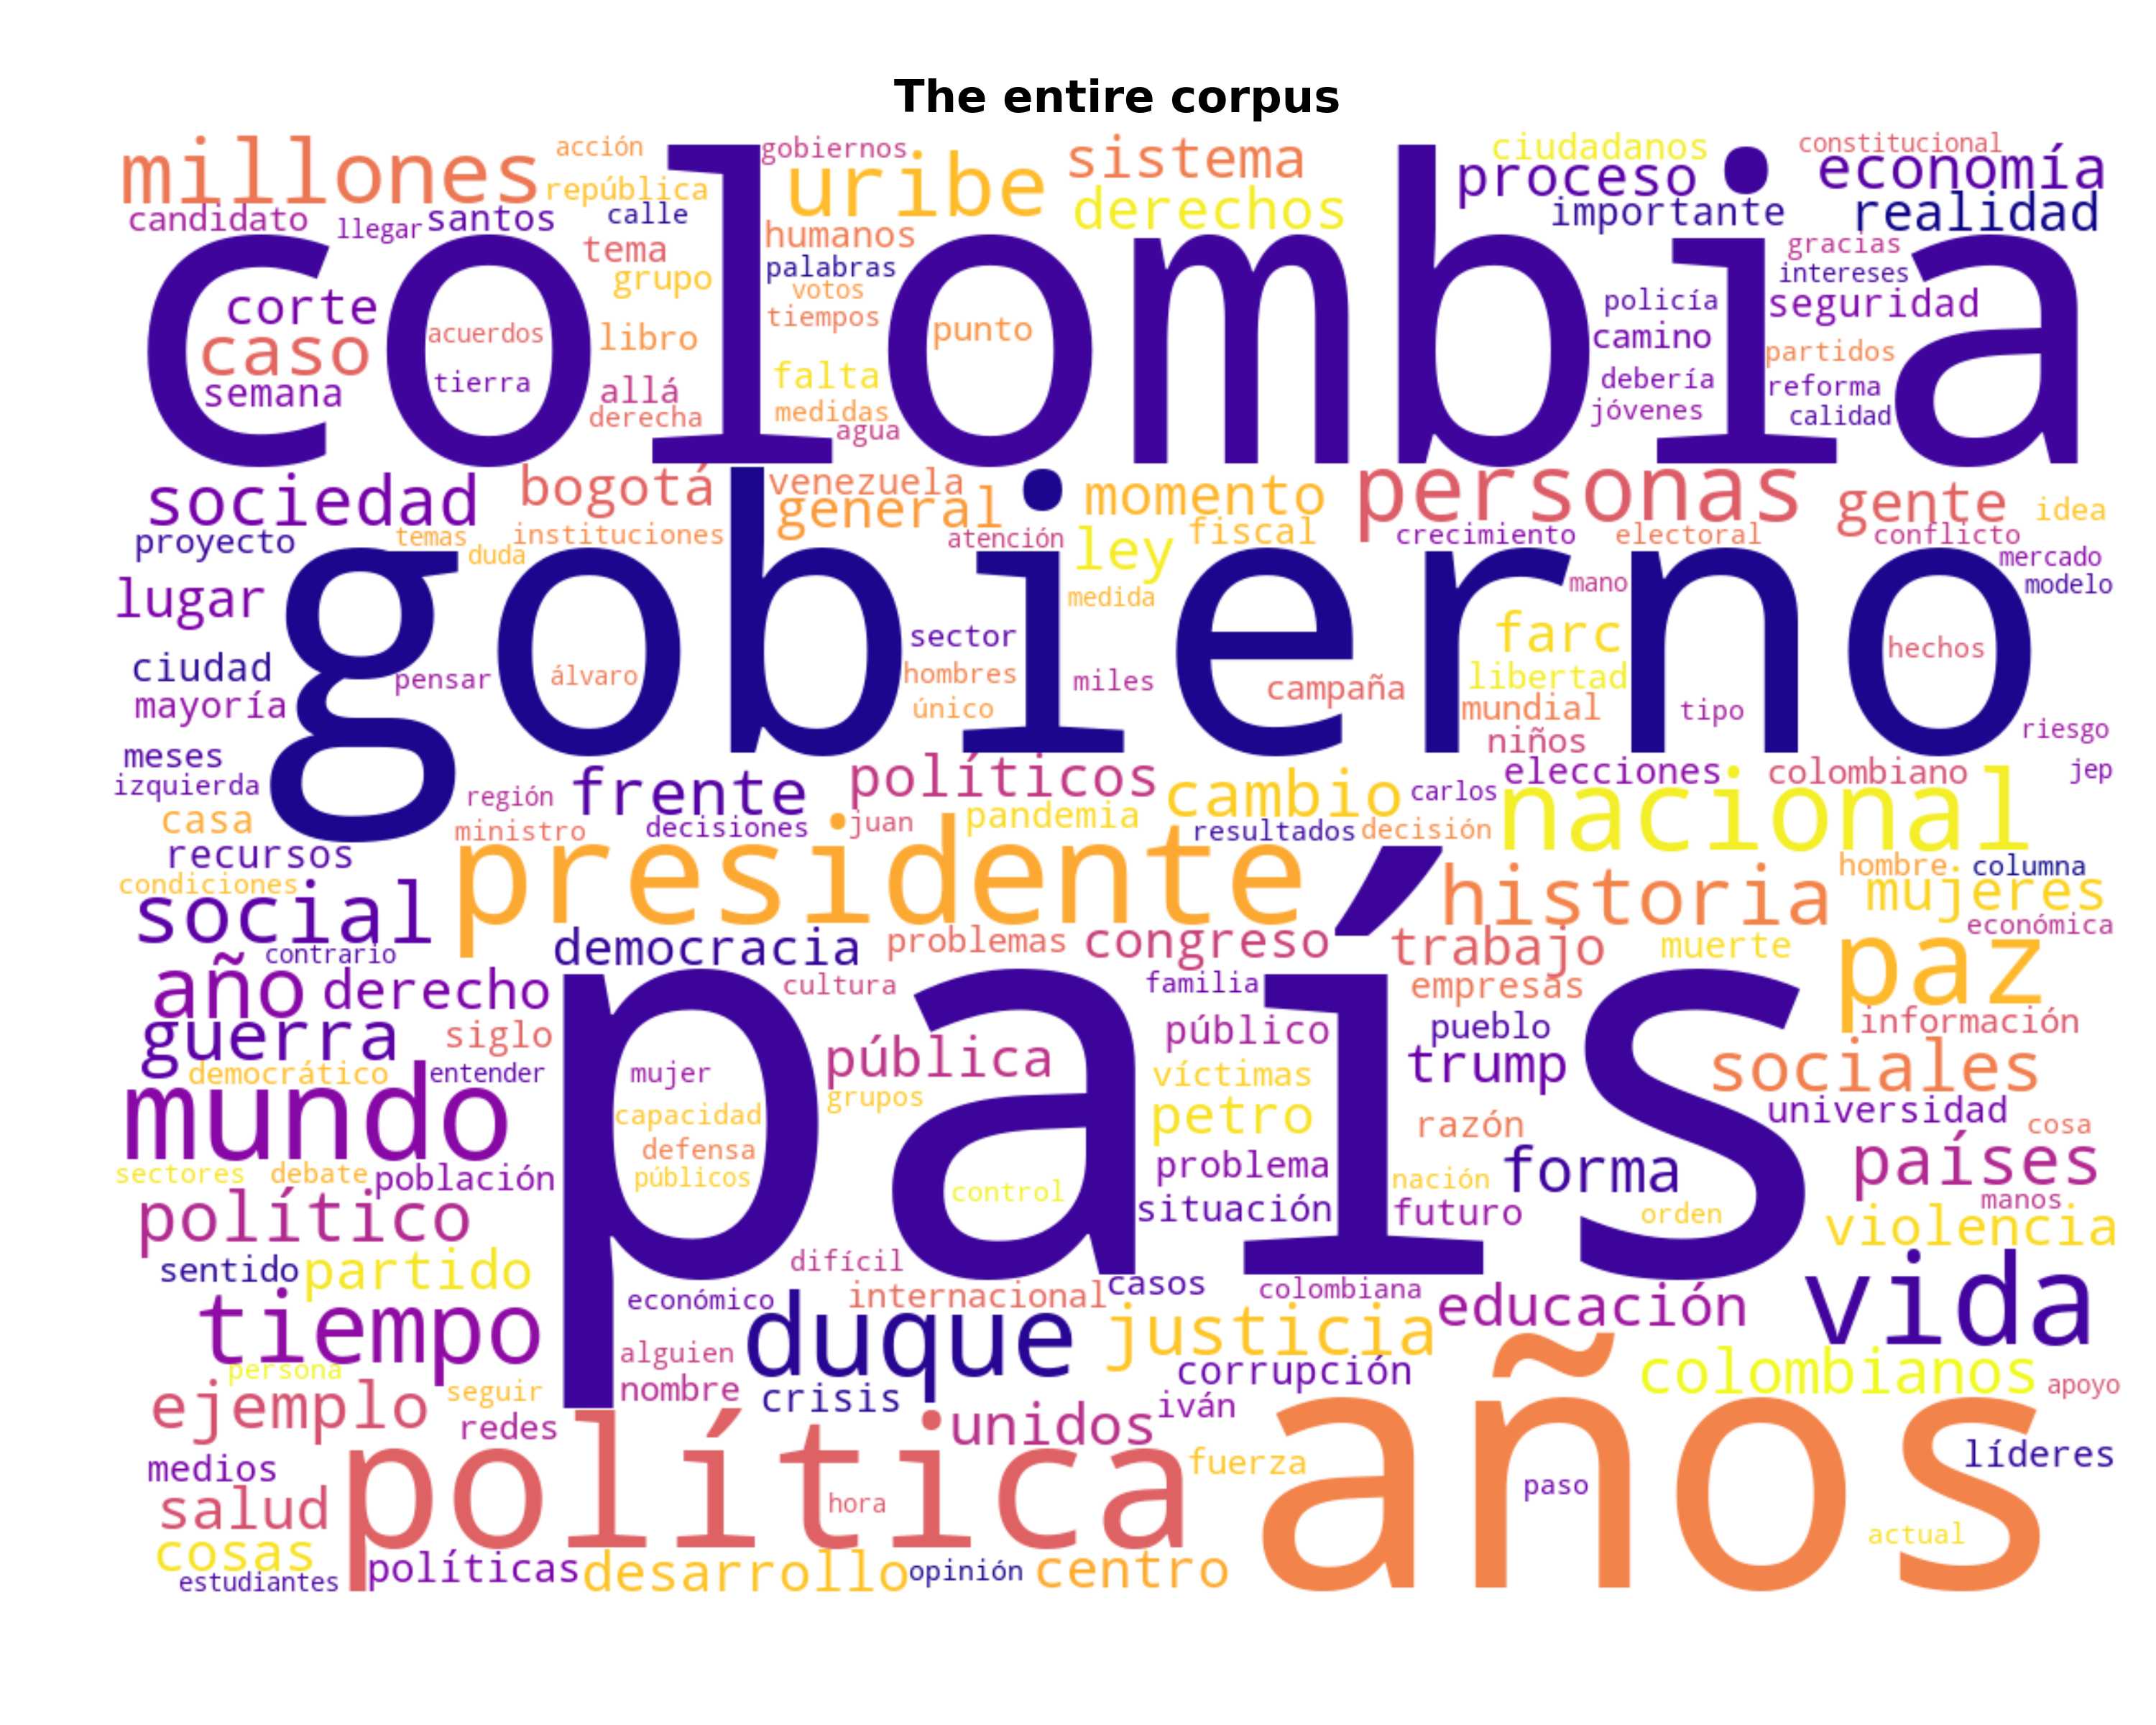
\includegraphics[width=\textwidth]{figures/nube_general.png}
			\caption{Nube de palabras corpus general}
			\label{fig:nube_general}
		\end{subfigure}
		\hfill
		\begin{subfigure}{0.48\textwidth}
			\centering
			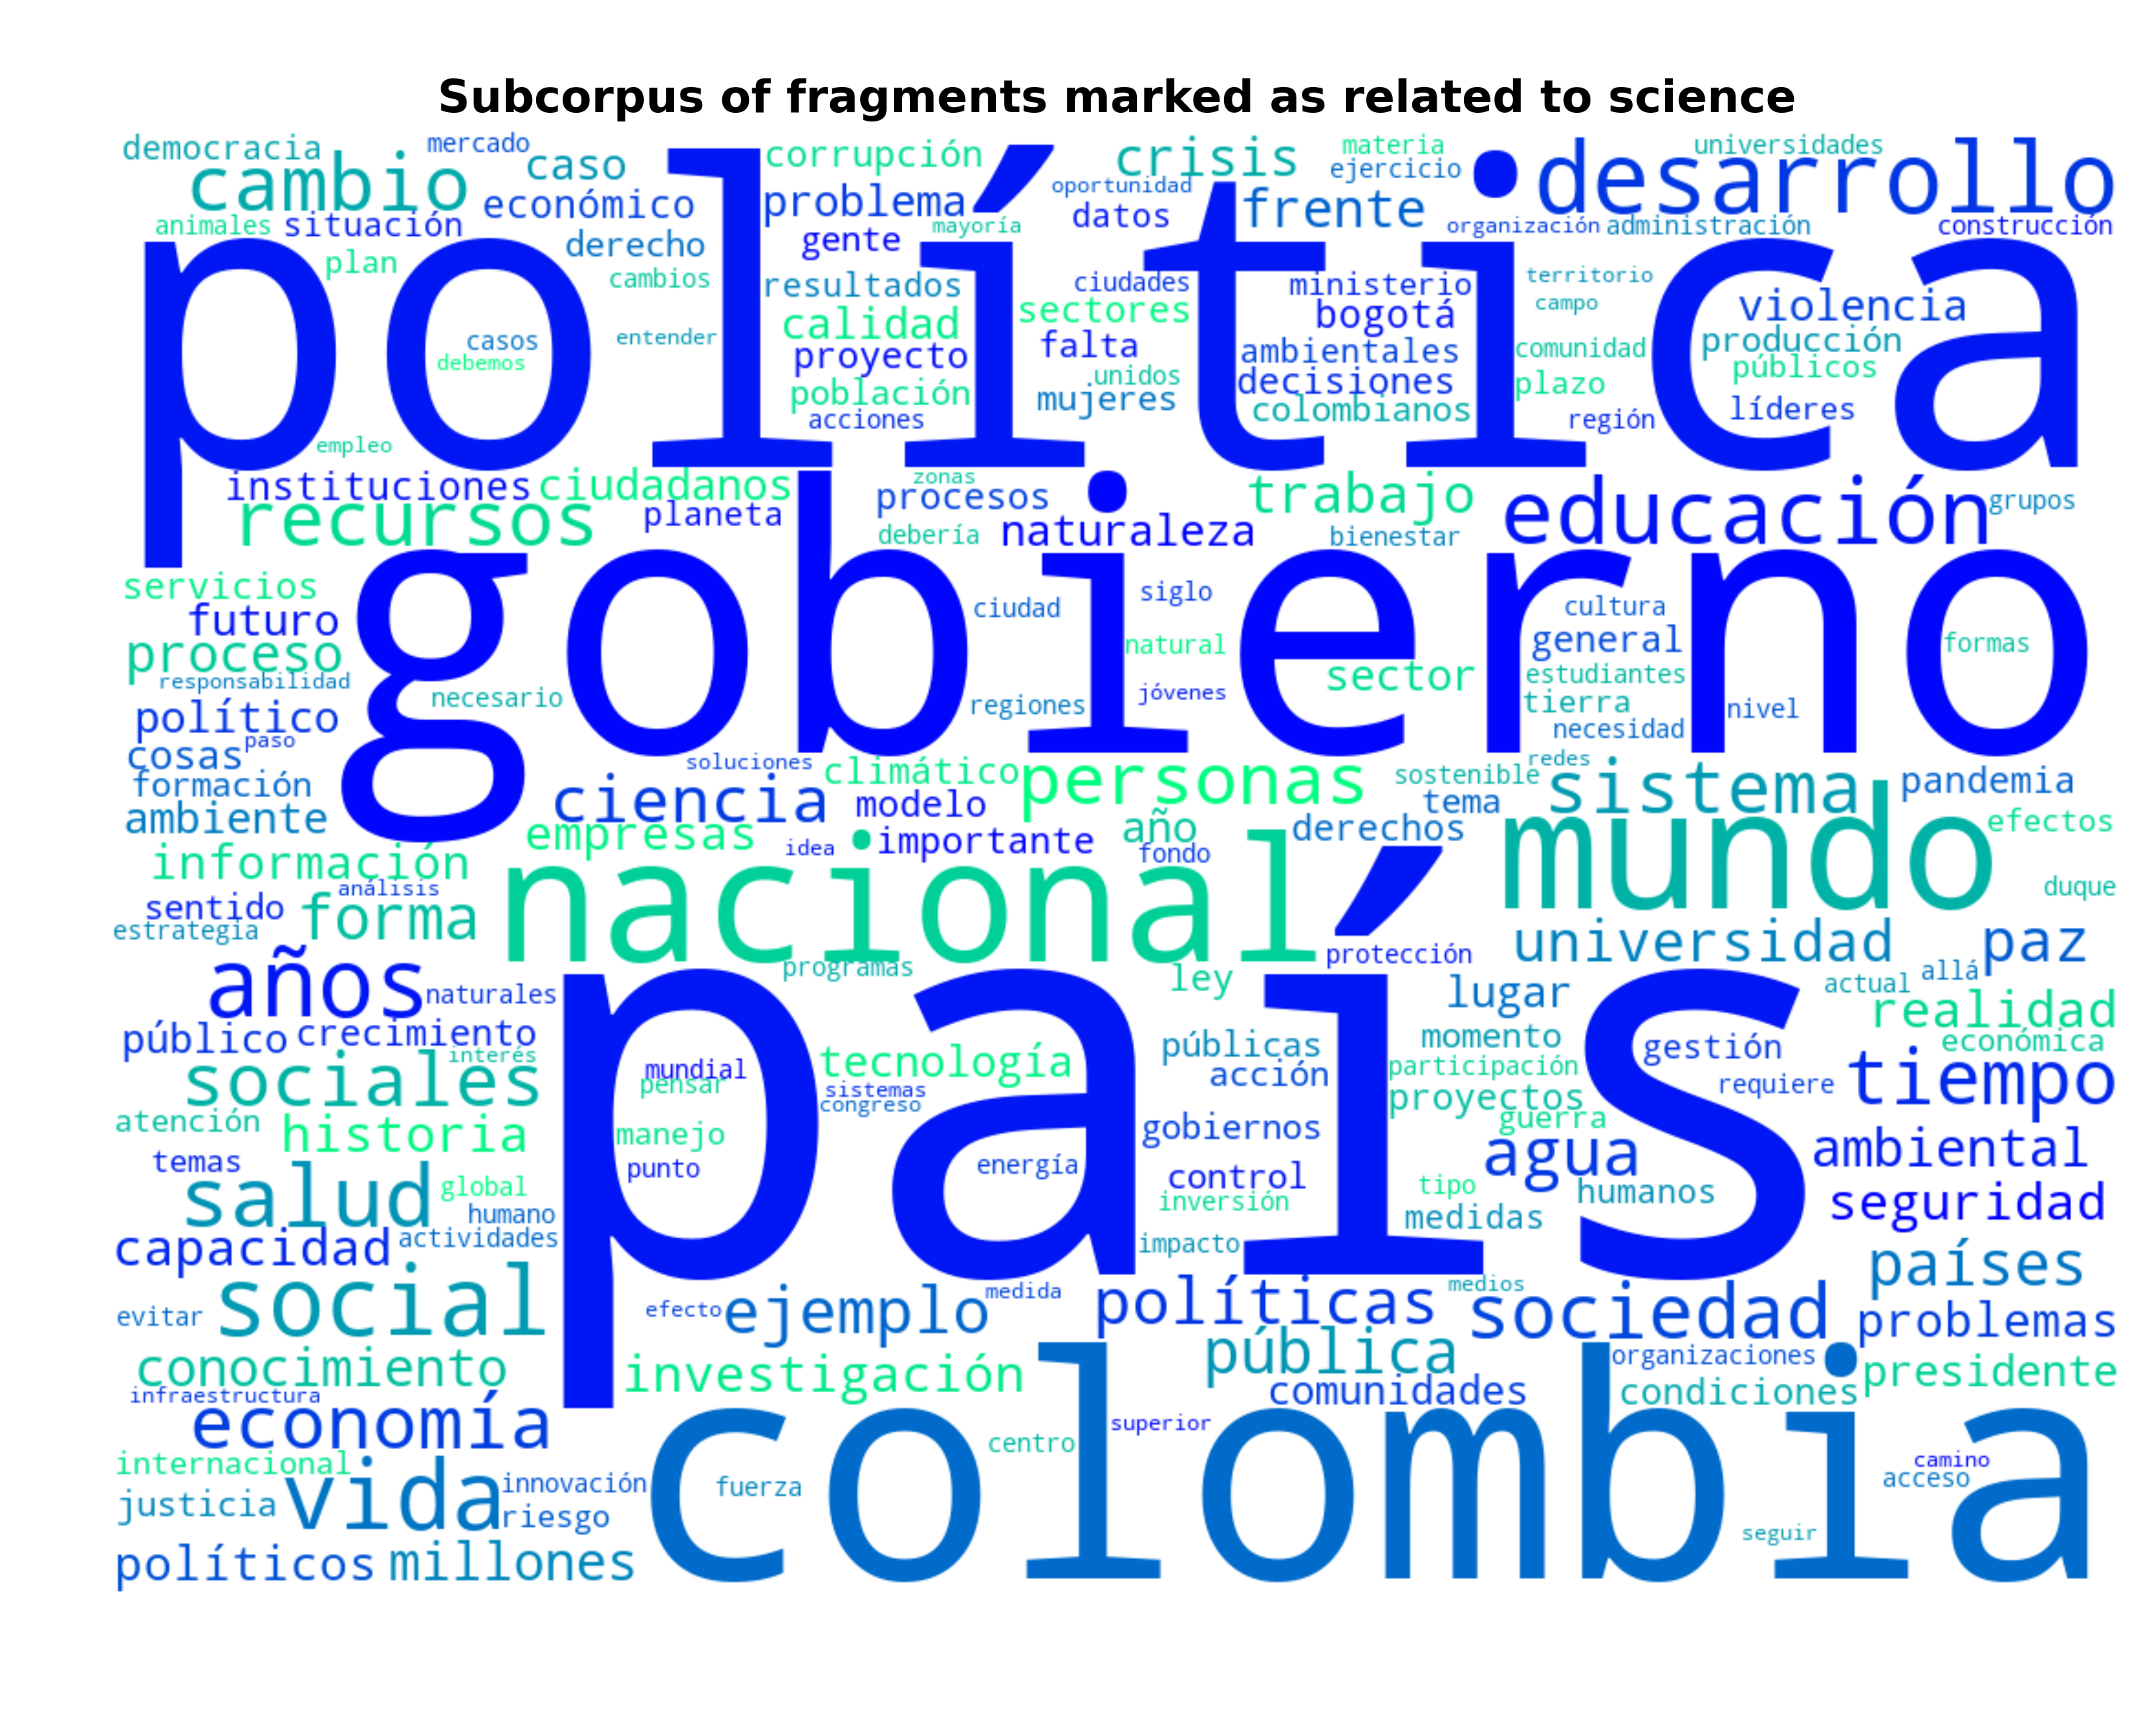
\includegraphics[width=\textwidth]{figures/nube_ciencia.png}
			\caption{Nube de palabras, fragmentos marcados como ciencia}
			\label{fig:nube_ciencia}
		\end{subfigure}
		\caption{Nubes de palabras}
		%\label{fig:resultados-clasificacion}
	\end{figure}
	


La Figura~\ref{fig:dist_mensual_ciencia} presenta, para cada mes del período analizado, el porcentaje de columnas que contienen al menos una mención efectiva a la ciencia respecto del total de columnas publicadas en ese mes. Esta representación permite observar la evolución temporal de la presencia del discurso científico en la opinión pública. Se aprecia un incremento notable en marzo y abril de 2020, meses en los que se concentra el mayor porcentaje de menciones, lo que sugiere una asociación directa entre la intensificación del discurso científico y el inicio de la pandemia de COVID-19.

	
	\begin{figure}[H]
		\centering
		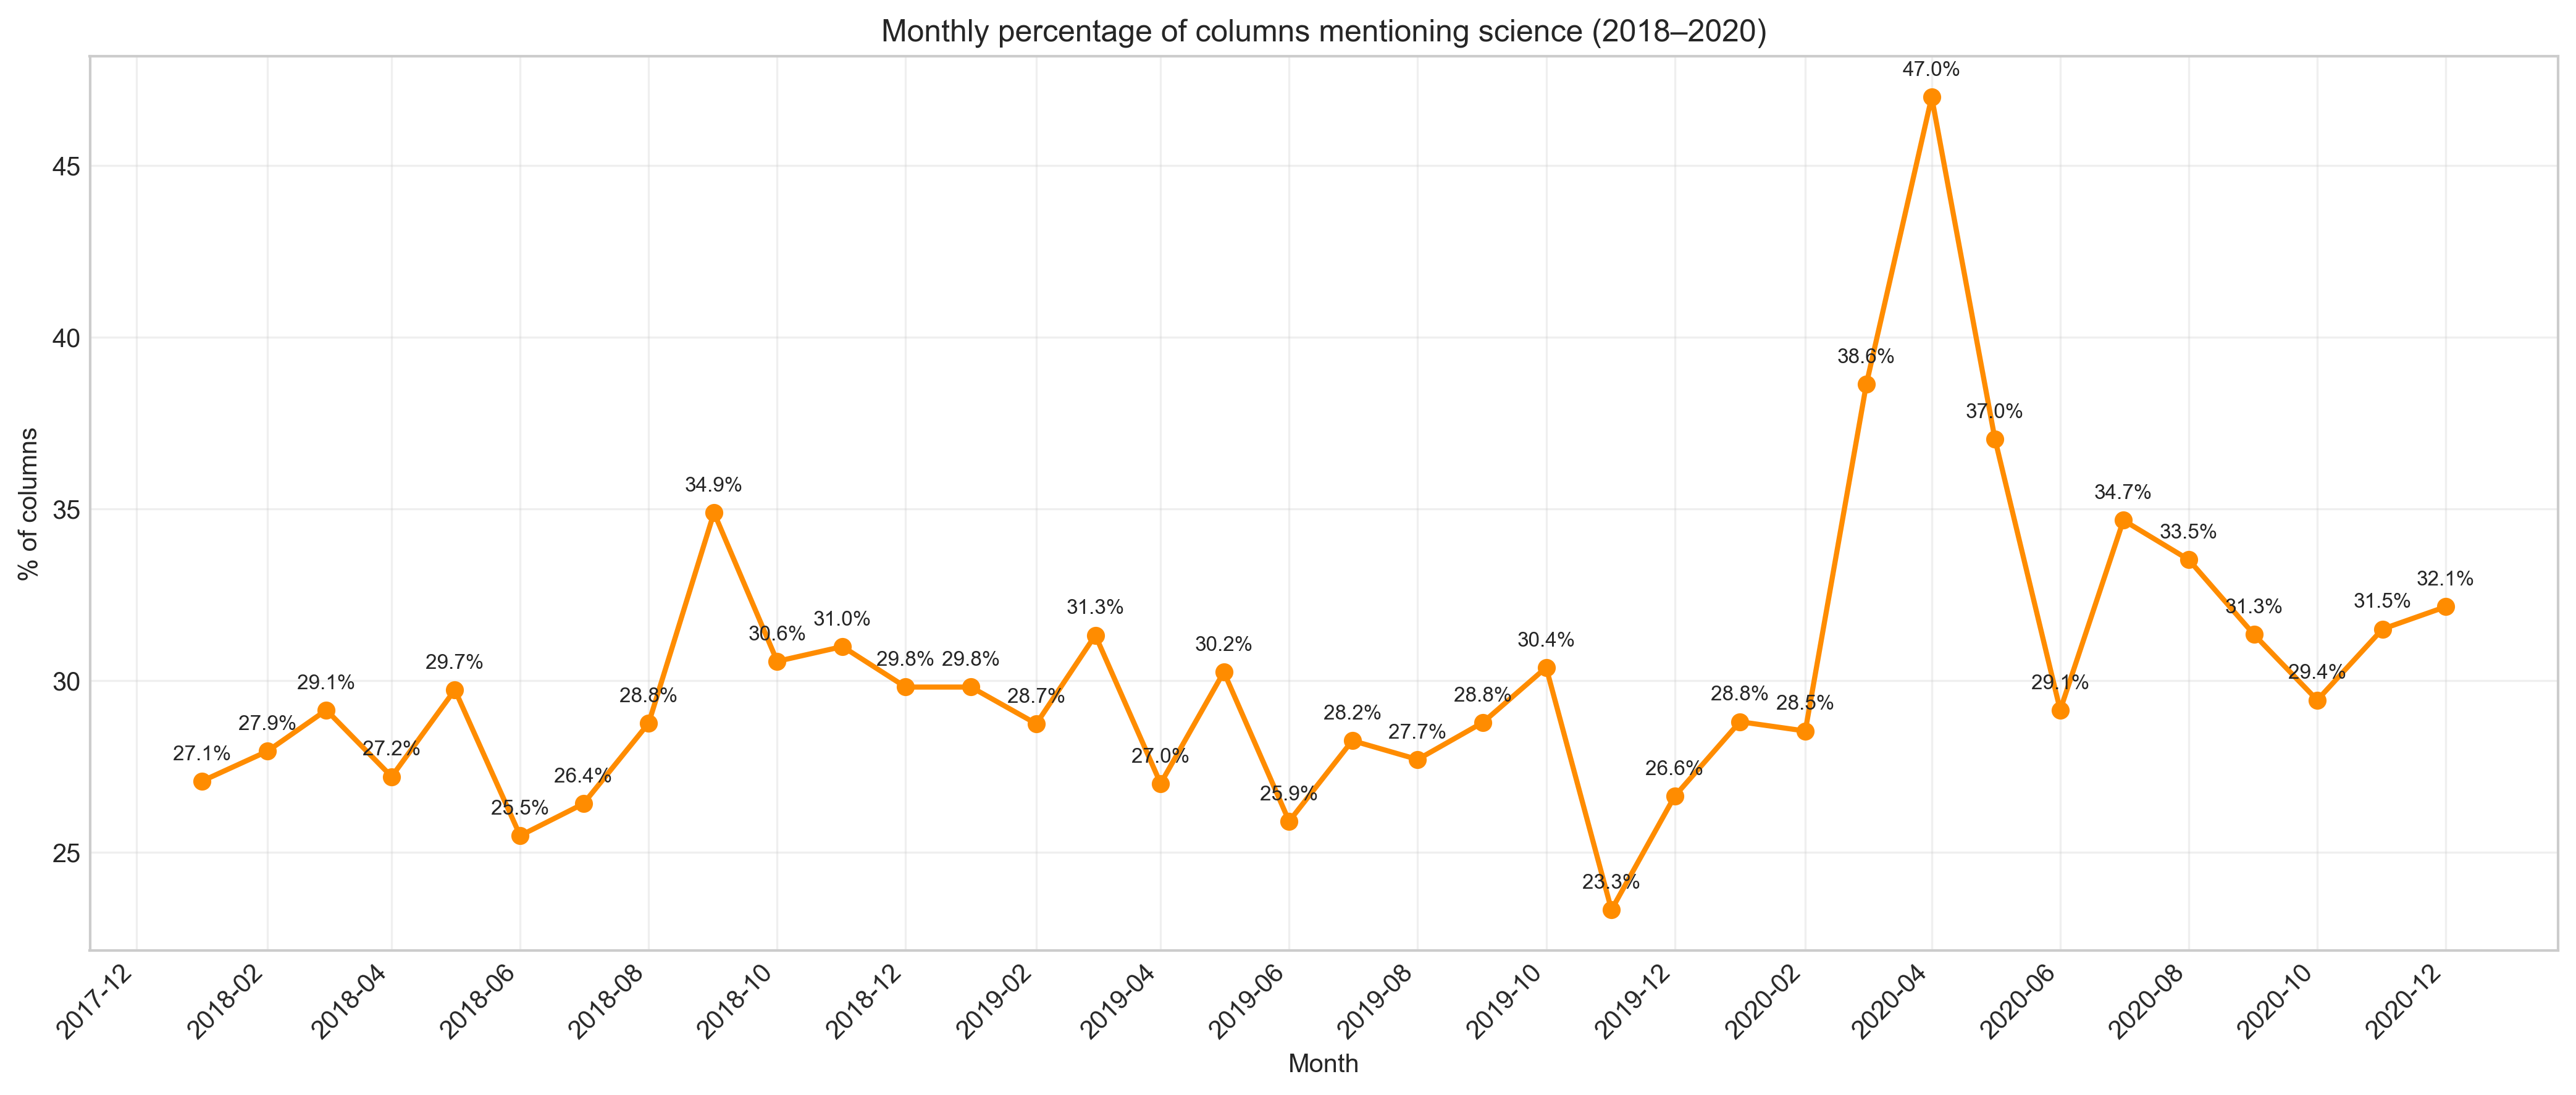
\includegraphics[width=0.95\textwidth]{figures/porcentaje_mensual_ciencia_linea.png}
		\caption{Distribución mensual de las columnas con menciones a la ciencia en porcentaje}
		\label{fig:dist_mensual_ciencia}
	\end{figure}
	
	
	
	\subsection{Reconocimiento de entidades nombradas}

A continuación se presentan las diez entidades más frecuentes por clase (Persona, Organización y Lugar), considerando únicamente aquellas cuya aparición supera el 30\% del subcorpus de fragmentos con mención efectiva a la ciencia. Este criterio permite concentrar el análisis en los actores, instituciones y espacios geográficos con mayor centralidad en el discurso científico de las columnas de opinión.
	
	

	\begin{table}[H]
		\centering
		\caption{Frecuencia comparativa de personajes en corpus general vs. corpus científico}
		\label{tab:ents_per}
		\footnotesize 

		\begin{tabular}{p{3cm}P{2.2cm}P{2.2cm}P{2.2cm}p{5cm}}
			\toprule
			\textbf{Entidad (PER)} & 
			\textbf{Frec. Corpus} & 
			\textbf{Frec. Ciencia} & 
			\textbf{\% Ciencia/ Corpus} & 
			\textbf{Descripción} \\
			\midrule
			Humboldt & 63 & 23 & 36 & Naturalista, geógrafo y explorador alemán, siglo XVIII y XIX. \\
			Newton & 25 & 9 & 36 & Físico inglés, siglos XVII y XVIII. \\
			Stephen Hawking & 41 & 16 & 39 & Científico y divulgador británico, siglos XX y XXI. \\
			Charles Darwin & 25 & 11 & 44 & Naturalista inglés, siglo XIX. \\
			Greta Thunberg & 50 & 16 & 32 & Activista ambiental sueca, siglo XXI. \\
			Ricardo Lozano & 15 & 7 & 46 & Geólogo y ex ministro de Ambiente y Desarrollo Sostenible de Colombia (2018). \\
			Mabel Torres & 13 & 7 & 53 & Científica colombiana y ex Ministra de Ciencia, Tecnología e Innovación de Colombia (2020) \\
			Wade Davis & 12 & 4 & 33 & Científico canadiense-colombiano. \\
			Dolly Montoya Castaño & 12 & 4 & 33 & Científica colombiana y ex rectora de la Universidad Nacional de Colombia. \\
			Carl Sagan & 10 & 5 & 50 & Astrónomo, astrofísico, divulgador estadounidense, siglo XX.\\
			
			\bottomrule
		\end{tabular}
	\end{table}
	
		\begin{table}[H]
		\centering
		\caption{Frecuencia comparativa de organizaciones en corpus general vs. corpus científico}
		\label{tab:ents_org}
		\footnotesize 
		
		\begin{tabular}{p{3cm}P{2.2cm}P{2.2cm}P{2.2cm}p{5cm}}
			\toprule
			\textbf{Entidad (ORG)} & 
			\textbf{Frec. Corpus} & 
			\textbf{Frec. Ciencia} & 
			\textbf{\% Ciencia/ Corpus} & 
			\textbf{Descripción} \\
			\midrule
			OCDE & 296 & 86 & 30 & Organización para la Cooperación y el Desarrollo Económico, organización internacional
			 \\
			Universidad Pedagógica Nacional & 117 & 55 & 47 & Universidad pública en Colombia \\
			Pontificia Universidad Javeriana & 103 & 33 & 32 & Universidad privada en Colombia. \\
			Ministerio de Agricultura & 111 & 33 & 30 & Ministerio de Colombia encargado del Sector Agropecuario, Pesquero y de Desarrollo Rural.  \\
			Colciencias & 74 & 47 & 63 & Anterior entidad encargada de promover las políticas públicas en ciencia, tecnología e innovación en Colombia. Reemplazada por Minciencias en 2019. \\
			Ministerio de Ambiente y Desarrollo Sostenible & 70 & 41 & 59 & Ministerio colombiano encargado de políticas en materia ambiental. \\
			Universidad de Massachusetts Amherst & 49 & 21 & 42 & Universidad pública y centro de investigación de Estados Unidos ubicada en Amherst, Massachusetts. \\
			Finagro & 44 & 15 & 34 & Fondo para el financiamiento del sector agropecuario, organización financiera en Colombia. \\
			IDEAM & 40 & 24 & 60 & Instituto de Hidrología, Meteorología y Estudios Ambientales de Colombia. \\
			FAO & 40 & 15 & 37 & Organización de las Naciones Unidas para la Alimentación y la Agricultura.\\
			
			\bottomrule
		\end{tabular}
	\end{table}
	
	\begin{table}[H]
		\centering
		\caption{Frecuencia comparativa de ubicaciones geográficas en corpus general vs. corpus científico}
		\label{tab:ents_loc}
		\footnotesize 
		\begin{tabular}{p{3cm}P{2.2cm}P{2.2cm}P{2.2cm}p{5cm}}
			\toprule
			\textbf{Entidad (LOC)} & 
			\textbf{Frec. Corpus} & 
			\textbf{Frec. Ciencia} & 
			\textbf{\% Ciencia/Corpus} & 
			\textbf{Descripción/Contexto} \\
			\midrule
			Amazonia & 306 & 112 & 37,21 & Región biogeográfica que comprende la selva tropical de la cuenca del Amazonas en Suramérica. \\
			Hidroituango & 127 & 46 & 36,22 & Proyecto hidroeléctrico en Antioquia, Colombia, sobre el río Cauca. \\
			Río Cauca & 93 & 33 & 32,58 & Segundo río más importante de Colombia, atraviesa la región andina. \\
			Orinoquia & 40 & 14 & 35,00 & Región natural de Colombia y Venezuela, también conocida como Llanos Orientales. \\
			Río Bogotá & 31 & 16 & 51,61 & Río que atraviesa la sabana de Bogotá, con importantes problemas de contaminación. \\
			Sabana & 28 & 13 & 46,43 & Referencia a la Sabana de Bogotá, altiplano en la cordillera Oriental. \\
			Parques Nacionales Naturales (PNN) & 35 & 15 & 33,33 & Sistema de áreas protegidas de Colombia, dependiente del Ministerio de Ambiente. \\
			Mar Caribe & 20 & 7 & 35,00 & Mar abierto tropical del océano Atlántico, baña las costas norte de Colombia. \\
			Mocoa & 18 & 9 & 50,00 & Ciudad capital del departamento de Putumayo, Colombia, en la región amazónica. \\
			\bottomrule
		\end{tabular}
	\end{table}
	
	
	\subsection{Modelado de tópicos}
Inicialmente, este ejercicio de modelado de tópicos se realizó sobre el corpus completo, con el propósito de caracterizar la estructura temática general de las columnas de opinión antes de focalizar el análisis en el subcorpus de ciencia. Para ello, se ejecutó el modelo variando el parámetro \textit{num\_topics}, que define el número máximo de tópicos que pueden estimarse. Cada configuración del parámetro produce un modelo distinto, entendido aquí como una estructura específica de agrupación semántica en la que los fragmentos del corpus se distribuyen en un conjunto determinado de tópicos latentes.

Para cada modelo estimado se calculó la métrica de coherencia \textit{c\_v}, la cual evalúa el grado de consistencia semántica interna de los términos más representativos de cada tópico. En términos generales, valores más altos de coherencia indican que las palabras que definen un tópico tienden a coocurrir en el corpus, lo que suele asociarse con una mayor interpretabilidad desde el punto de vista humano. Reportar los resultados para distintas configuraciones permite comparar la calidad temática de los modelos y fundamentar la selección del número de tópicos más adecuado.

\textcolor{red}{Los resultados obtenidos se presentan en la Tabla~\ref{tab:coherence_topics}.}

\begin{table}[H]
	\centering
	\begin{tabular}{ccccc}
		\hline
		\textbf{num\_topics} & \textbf{num\_topics\_final} & \textbf{coherence\_c\_v} & \textbf{\% outliers} \\
		\hline
		auto & 63 & 0.681289 & 0.0 \\
		60   & 59 & 0.671076 & 0.0 \\
		30   & 29 & 0.652175 & 0.0 \\
		40   & 39 & 0.635335 & 0.0 \\
		20   & 19 & 0.545472 & 0.0 \\
		10   & 9  & 0.480771 & 0.0 \\
		\hline
	\end{tabular}
	\caption{Resultados del modelado de tópicos para distintos valores del parámetro \textit{num\_topics}}
	\label{tab:coherence_topics}
\end{table}

El número de tópicos finales es menor en una unidad respecto al valor inicialmente definido por el parámetro, ya que al aplicar la reducción de \emph{outliers} se elimina el tópico que agrupa los documentos considerados atípicos. Se observa que, en general, al aumentar el número máximo de tópicos, el valor de coherencia tiende a incrementarse, lo que sugiere una mayor homogeneidad semántica dentro de cada agrupación. En particular, cuando el modelo determina automáticamente el número de tópicos, se obtienen 63 tópicos finales y el mayor valor de coherencia entre las configuraciones evaluadas.

		
Manteniendo el modelo de 63 tópicos, en la tabla \ref{tab:bertopic_coherence_top} se presentan los 10 tópicos con mayor porcentaje de documentos agrupados, junto con el valor de coherencia calculado para cada uno y sus respectivas palabras representativas. En conjunto, estos 10 tópicos concentran el 70\% de los fragmentos analizados.
		
		\begin{table}[H]
			\centering
			\small
			\begin{tabularx}{\textwidth}{c c c X}
				\hline
				\textbf{Topic} & \textbf{Coherence  ($c_v$)} & \textbf{Percentage (\%)} & \textbf{Keywords} \\
				\hline
				0  & 0.5509 & 40.06 & presidente, gobierno, duque, paz, país, uribe, colombia, política, años, petro \\
				2  & 0.8437 & 5.58  & economía, impuestos, crecimiento, ingresos, fiscal, empresas, tasa, empleo, pib, déficit \\
				1  & 0.7322 & 5.27  & pandemia, virus, salud, coronavirus, covid19, mundo, cuarentena, medidas, crisis, personas \\
				3  & 0.8185 & 4.25  & educación, estudiantes, universidad, universidades, calidad, formación, superior, nacional, profesores, colegios \\
				4  & 0.8427 & 3.34  & mujeres, mujer, hombres, sexual, violencia, género, sexo, feminismo, acoso, sexuales \\
				7  & 0.6890 & 2.53  & redes, información, datos, facebook, medios, sociales, comunicación, personas, internet, twitter \\
				8  & 0.7879 & 2.23  & hectáreas, rural, deforestación, tierras, agricultura, productores, agropecuario, cultivos, \textcolor{green}{000}, desarrollo \\
				5  & 0.8642 & 2.13  & fútbol, jugadores, equipo, juego, equipos, copa, selección, deporte, gol, mundial \\
				20 & 0.5990 & 2.05  & corrupción, corruptos, públicos, consulta, anticorrupción, lucha, funcionarios, recursos, país, política \\
				6  & 0.8998 & 1.61  & cocina, comida, comer, restaurante, plato, sabores, arroz, platos, sabor, casa \\
				\hline
			\end{tabularx}
			\caption{Top tópicos de BERTopic con coherencia por tópico ($c_v$), porcentaje de documentos y palabras representativas}
			\label{tab:bertopic_coherence_top}
		\end{table}
		
		El mismo procedimiento fue aplicado a los fragmentos clasificados como menciones a la ciencia. 
		
		\begin{table}[H]
			\centering
			\begin{tabular}{c c c c}
				\hline
				\textbf{num\_topics} & \textbf{num\_topics\_final} & \textbf{Coherence $c_v$} & \textbf{\% Outliers} \\
				\hline
				20   & 19 & 0.695491 & 0.0 \\
				40   & 28 & 0.695162 & 0.0 \\
				auto & 26 & 0.694176 & 0.0 \\
				30   & 28 & 0.681233 & 0.0 \\
				60   & 27 & 0.678842 & 0.0 \\
				10   & 9  & 0.622583 & 0.0 \\
				\hline
			\end{tabular}
			\caption{Resultados de BERTopic para distintos valores de \texttt{num\_topics}, especifico ciencia}
			\label{tab:bertopic_nr_topics_ciencia}
		\end{table}
		
		En este caso, el mejor modelo entre los evaluados fue el de 20 tópicos, de acuerdo con la métrica utilizada. Para este modelo, los resultados se presentan en la Tabla \ref{tab:topics_ciencia}. Asimismo, se observa que el 90\% de los documentos se concentró en los 10 primeros tópicos, lo que indica una alta concentración temática en un subconjunto reducido de tópicos.
		
		\begin{table}[H]
			\centering
			\small
			\begin{tabularx}{\textwidth}{c c c X}
				\hline
				\textbf{Topic} & \textbf{Coherence ($c_v$)} & \textbf{Percentage (\%)} & \textbf{Keywords} \\
				\hline
				1  & 0.493785 & 25.62 & política, gobierno, paz, país, seguridad, violencia, político, políticos, justicia, colombia \\
				0  & 0.460526 & 21.69 & salud, mundo, vida, pandemia, tiempo, ciencia, personas, virus, años, crisis \\
				3  & 0.574302 & 11.42 & economía, desarrollo, crecimiento, recursos, país, sector, gobierno, política, fiscal, innovación \\
				2  & 0.782987 & 9.61  & educación, universidad, formación, universidades, estudiantes, nacional, calidad, investigación, conocimiento, superior \\
				4  & 0.784604 & 6.56  & ambiental, ambientales, conservación, ambiente, biodiversidad, sostenible, desarrollo, deforestación, bosques, ecosistemas \\
				5  & 0.799532 & 4.79  & climático, cambio, planeta, global, calentamiento, incendios, mundo, climática, clima, temperatura \\
				8  & 0.504077 & 2.79  & datos, información, encuestas, acceso, transparencia, resultados, personas, medios, ejemplo, pública \\
				7  & 0.686045 & 2.75  & agua, río, aguas, lluvia, ríos, cauca, barrios, obras, bogotá, país \\
				9  & 0.919135 & 2.02  & energía, combustibles, fósiles, energías, carbón, renovables, solar, energética, petróleo, gas \\
				10 & 0.724657 & 1.83  & mujeres, hombres, mujer, género, femenino, violencia, personas, vida, femenina, sexo \\
				\hline
			\end{tabularx}
			\caption{Top tópicos de BERTopic con coherencia por tópico ($c_v$), porcentaje de documentos y palabras representativas, específico para menciones a ciencia}
			\label{tab:topics_ciencia}
		\end{table}
		
		
		
	\subsection{Análisis de vocabulario con POS-tagging}

Se extrajeron los verbos, adjetivos y sustantivos del corpus mediante técnicas de \emph{POS-tagging} y se calcularon sus frecuencias. En total, se identificaron aproximadamente 10 mil verbos, 18 mil adjetivos y 30 mil sustantivos distintos. En el corpus completo, el verbo más frecuente es \textit{tener}, el adjetivo más frecuente es \textit{social} y el sustantivo más frecuente es \textit{país}. Estas mismas palabras encabezan también las listas de frecuencia en el subcorpus de fragmentos con mención efectiva a la ciencia.

Dado que el 11.6\% de los fragmentos del corpus fueron clasificados como menciones científicas (véase sección \ref{sec:ident_menciones}), se seleccionaron aquellas palabras cuya proporción de ocurrencia en el subcorpus de ciencia supera ese porcentaje. Este criterio permite identificar términos con una presencia relativamente mayor en el discurso científico en comparación con el corpus general. A partir de este filtro se obtuvo el conjunto final de palabras analizadas en esta sección.



\begin{table}[H]
	\centering
	\begin{tabular}{lrrr}
		\toprule
		\textbf{Verbo} & \textbf{Frecuencia total} & \textbf{Frecuencia ciencia} & \textbf{Proporción ciencia} \\
		\midrule
		articular     & 175 & 79 & 0.45 \\
		mitigar       & 208 & 68 & 0.33 \\
		contaminar    & 200 & 63 & 0.32 \\
		gestionar     & 188 & 57 & 0.30 \\
		actualizar    & 122 & 37 & 0.30 \\
		deforestar    & 67  & 26 & 0.39 \\
		posibilitar   & 77  & 24 & 0.31 \\
		apalancar     & 54  & 22 & 0.41 \\
		planificar    & 43  & 20 & 0.47 \\
		capacitar     & 46  & 20 & 0.43 \\
		dinamizar     & 62  & 20 & 0.32 \\
		armonizar     & 47  & 19 & 0.40 \\
		maximizar     & 62  & 19 & 0.31 \\
		optimizar     & 39  & 18 & 0.46 \\
		cuantificar   & 47  & 18 & 0.38 \\
		almacenar     & 47  & 18 & 0.38 \\
		talar         & 39  & 17 & 0.44 \\
		\bottomrule
	\end{tabular}
	\caption{Frecuencia y proporción de verbos en el subcorpus de ciencia}
	\label{tab:verbos_ciencia}
\end{table}


\begin{table}[H]
	\centering
	\begin{tabular}{lrrr}
		\toprule
		\textbf{Adjetivo} & \textbf{Frecuencia total} & \textbf{Frecuencia ciencia} & \textbf{Proporción ciencia} \\
		\midrule
		ecosistémico & 65   & 53  & 0.82 \\
		invernadero  & 100  & 68  & 0.68 \\
		silvestre    & 133  & 81  & 0.61 \\
		hídrico      & 107  & 65  & 0.61 \\
		forestal     & 173  & 105 & 0.61 \\
		ambiental    & 1530 & 910 & 0.59 \\
		climático    & 984  & 584 & 0.59 \\
		renovable    & 149  & 84  & 0.56 \\
		fósil        & 196  & 110 & 0.56 \\
		ecológico    & 322  & 180 & 0.56 \\
		científico   & 959  & 507 & 0.53 \\
		energético   & 227  & 119 & 0.52 \\
		biológico    & 183  & 87  & 0.48 \\
		sostenible   & 744  & 342 & 0.46 \\
		animal       & 188  & 84  & 0.45 \\
		\bottomrule
	\end{tabular}
	\caption{Frecuencia y proporción de adjetivos en el subcorpus de ciencia}
	\label{tab:adjetivos_ciencia}
\end{table}

\begin{table}[H]
	\centering
	\begin{tabular}{lrrr}
		\toprule
		\textbf{Sustantivo} & \textbf{Frecuencia total} & \textbf{Frecuencia ciencia} & \textbf{Proporción ciencia} \\
		\midrule
		agua          & 2586 & 971 & 0.38 \\
		ciencia       & 1575 & 858 & 0.54 \\
		conocimiento  & 1753 & 665 & 0.38 \\
		tecnología    & 1547 & 622 & 0.40 \\
		naturaleza    & 1537 & 480 & 0.31 \\
		impacto       & 1419 & 462 & 0.33 \\
		formación     & 1124 & 412 & 0.37 \\
		ambiente      & 1256 & 398 & 0.32 \\
		gestión       & 1164 & 380 & 0.33 \\
		planeta       & 1207 & 379 & 0.31 \\
		energía       & 968  & 363 & 0.38 \\
		innovación    & 604  & 333 & 0.55 \\
		bosque        & 701  & 326 & 0.47 \\
		bienestar     & 1051 & 321 & 0.31 \\
		área          & 1037 & 314 & 0.30 \\
		\bottomrule
	\end{tabular}
	\caption{Frecuencia y proporción de sustantivos en el subcorpus de ciencia}
	\label{tab:sustantivos_ciencia}
\end{table}

	
	\section{Discusión}
	
Los métodos aplicados permitieron identificar y caracterizar elementos del discurso relacionados con la ciencia en columnas de opinión colombianas. A partir de la estrategia basada en procesamiento de lenguaje natural y del uso del tesauro de la UNESCO como marco conceptual, fue posible detectar fragmentos textuales con distintos grados de asociación a la ciencia y construir un subcorpus específico para su análisis.

No obstante, este enfoque presenta limitaciones inherentes a la forma en que se operacionaliza el concepto de ciencia a partir de listas de términos y medidas de similitud semántica. En particular, el método puede generar errores de clasificación, tanto falsos positivos como falsos negativos. En este sentido, la precisión máxima alcanzada (74 \%) indica un desempeño aceptable para un análisis exploratorio a gran escala, aunque también evidencia la necesidad de interpretar los resultados con cautela y de considerar mejoras metodológicas en trabajos futuros, por ejemplo mediante conjuntos de validación más amplios o esquemas híbridos de anotación automática y manual.

%Un aporte relevante del uso del tesauro de la UNESCO es la posibilidad de desagregar las menciones a la ciencia en categorías temáticas, lo que permite un primer acercamiento sistemático a los temas científicos que circulan en el discurso público. Los resultados muestran que una proporción significativa de los fragmentos identificados se concentra en la categoría Administración de la ciencia y de la investigación (43 \%), seguida por Polución, catástrofes y seguridad (21 \%). Esta distribución sugiere que, en las columnas de opinión analizadas, la ciencia aparece principalmente asociada a debates sobre su gestión institucional, las políticas públicas en ciencia y tecnología, y a coyunturas críticas vinculadas con riesgos, crisis y problemáticas socioambientales.

La distribución presentada en la Tabla~\ref{tab:res_fragmentos_subcategoria} evidencia una marcada concentración temática: casi la mitad de los fragmentos con mención a la ciencia se ubican en la categoría Administración de la ciencia y de la investigación (43.97\%), seguida por Polución, catástrofes y seguridad (21.55\%). Este patrón sugiere que la ciencia, en el discurso de opinión analizado, aparece principalmente vinculada a su dimensión institucional y política (financiación, gestión, políticas públicas) y a contextos de crisis y riesgo socioambiental. En contraste, las disciplinas científicas específicas (como ciencias físicas, químicas o de la tierra) ocupan un lugar mucho menos visible.

Esta asimetría indica que la ciencia no circula en la esfera pública como un conjunto equilibrado de saberes disciplinares, sino como un campo asociado a debates coyunturales e institucionales. No obstante, debe considerarse que las categorías del Tesauro poseen distinta amplitud conceptual, lo que podría influir en su frecuencia relativa. Aun así, la concentración observada apunta de manera consistente a una representación pública de la ciencia centrada más en su gobernanza y en situaciones críticas que en la discusión técnica especializada.


Este patrón temático se refuerza al considerar su dimensión temporal. Como se observa en la Figura~\ref{fig:dist_mensual_ciencia}, los mayores picos en la proporción de columnas con menciones a la ciencia se registran en marzo y abril de 2020, coincidiendo con el inicio de la pandemia por COVID-19. En abril de 2020 se alcanza el valor máximo del período analizado, lo que evidencia un aumento sustancial en la visibilidad pública de la ciencia. Durante estos meses, la ciencia y los científicos adquieren un lugar central en el debate público, particularmente en relación con decisiones gubernamentales, medidas sanitarias y gestión del riesgo.

En cuanto a los actores y organizaciones mencionados en los fragmentos asociados a la ciencia (ver Tablas~\ref{tab:ents_per},\ref{tab:ents_org},\ref{tab:ents_loc}), los resultados del reconocimiento de entidades muestran una predominancia de científicos ampliamente reconocidos, activistas ambientales y científicos colombianos que han ocupado cargos políticos o posiciones en ministerios. En el plano organizacional, destacan organismos de cooperación internacional vinculados al desarrollo, ministerios responsables de la administración de la ciencia, el ambiente y el desarrollo sostenible en Colombia, así como universidades nacionales e internacionales. Este conjunto de entidades sugiere que la ciencia, en las columnas de opinión, aparece estrechamente ligada tanto a estructuras institucionales del Estado como a redes académicas y organismos internacionales, reforzando su carácter político e institucional en la esfera pública.

A partir del modelado de tópicos aplicado al subcorpus de fragmentos con menciones a la ciencia (véase Tabla~\ref{tab:topics_ciencia}), se identifican varios ejes temáticos claramente diferenciados. El tópico con mayor proporción (25.62\%) se articula en torno a categorías políticas e institucionales (política, gobierno, paz, seguridad), lo que sugiere que la ciencia aparece frecuentemente integrada en debates de carácter público y gubernamental más amplios. En segundo lugar (21.69\%), emerge un tópico asociado a salud y pandemia (salud, virus, crisis, ciencia), confirmando que la coyuntura del COVID-19 desempeñó un papel central en la visibilidad del discurso científico. También se identifican tópicos relevantes vinculados al desarrollo económico (11.42\%) y a la educación e investigación (9.61\%), lo que indica una conexión entre ciencia, innovación y formación superior. En el ámbito ambiental, aparecen de manera diferenciada tópicos relacionados con conservación y biodiversidad (6.56\%), cambio climático (4.79\%), recursos hídricos (2.75\%) y energía (2.02\%), lo que refuerza la idea de que las problemáticas ambientales constituyen un eje estructural en la articulación entre ciencia y opinión pública. En conjunto, estos resultados muestran que la ciencia no se presenta exclusivamente como contenido técnico especializado, sino como un recurso discursivo que atraviesa debates políticos, económicos, educativos y ambientales.


El análisis del vocabulario refuerza y complementa los hallazgos del modelado de tópicos. En el caso de los adjetivos, predominan aquellos asociados al ámbito ambiental y climático, como ambiental, climático, ecosistémico o renovable, lo que indica que la ciencia es caracterizada principalmente a partir de problemáticas ecológicas y de sostenibilidad. Por su parte, los sustantivos más representativos se vinculan con conceptos como tecnología, conocimiento, naturaleza, formación y gestión, lo que sugiere una concepción de la ciencia orientada tanto a la producción de saberes como a su aplicación práctica y a su administración institucional.

En cuanto a los verbos, resulta particularmente relevante la alta frecuencia de articular, lo cual apunta a una representación de la ciencia como un elemento que debe ser conectado con otros ámbitos, tales como la política pública, el desarrollo económico, la educación o la gestión ambiental. De manera similar, verbos como mitigar adquieren un papel central en contextos relacionados con la reducción de los efectos del calentamiento global, la degradación ambiental o la propagación de enfermedades, evidenciando una narrativa en la que la ciencia aparece como una herramienta para enfrentar riesgos y crisis. Finalmente, la recurrencia de verbos como gestionar, planificar y optimizar refuerza la idea de una ciencia concebida no solo como producción de conocimiento abstracto, sino como un recurso estratégico orientado a la toma de decisiones, la eficiencia y la intervención sobre problemas sociales y ambientales.

En conjunto, estos resultados sugieren que, en las columnas de opinión colombianas, la ciencia es representada predominantemente desde una perspectiva instrumental y contextualizada, estrechamente vinculada a coyunturas críticas, desafíos ambientales y procesos de gobernanza, más que como un conjunto de disciplinas abstractas o saberes descontextualizados.
	
	
	\section{Limitaciones y consideraciones éticas}
	Cobertura mediática, sesgos de autoría/medio, ambigüedad semántica, cumplimiento de TOS/licencias, privacidad y reproducibilidad.
	
	\section{Reproducibilidad y datos}
	Enlace a repositorio (GitHub/OSF/Zenodo), scripts, versión de paquetes y \emph{conteiner} (\texttt{Dockerfile}) si aplica. 
	Describe estructura del repo y cómo reproducir figuras/tablas.
	
	\section{Conclusiones y trabajo futuro}
	Síntesis de aportes y próximos pasos (ampliar periodos, añadir encuestas, enriquecer anotaciones, análisis multilingüe, etc.).
	
	\section*{Agradecimientos}
	Reconocimientos a colaboradores, financiación, y fuentes de datos.
	
	% --- Bibliografía ---
	\bibliography{references}  % Crea un archivo references.bib con tus entradas
	

	
	
	% --- Apéndices (opcional) ---
	\appendix

	
\end{document}
